\chapter{Свойства многослойных сферических маскирующих
  покрытий} \label{chapt3}
\section{Введение}
В течение последнего десятилетия наблюдается сильный интерес к
тематике метаматериалов, искусственной среды с экзотическими
электромагнитными свойствами~\cite{Smith-2004,
  Schurig-2006, Shalaev-2007, Kivshar-2012}. Одним из самых известных
применений метаматериалов является маскировка. Как правило,
маскирующие покрытия разрабатываются с использованием концепции
трансформационной оптики~\cite{pendry_TO, Leonhardt-2006} и
используют метаматериалы с анизотропными, магнитными и экстремальными
материальными параметрами. Из-за искусственной природы этой среды
экспериментальная реализация маскировки является нетривиальной,
особенно для случая работы в диапазоне оптических
частот~\cite{Kildishev:2011, alu, XU-Su:120408, Alu-2005}. 

Недавно было предпринято несколько попыток достичь маскировки с
использованием натуральных изотропных диэлектрических материалов. В
работах~\cite{Sigmund-AllDiel-2011, smith-3dprinterCloak-2013,
  Fujii_topolOpti_theory_2013,
  ma-experiment-topology-2013,LayeredShell,MOP:MOP27024} были
предложены устройства маскировки со сложной геометрией, полученной
с помощью численной оптимизации, выполненные с использованием всего
одного вида диэлектрического материала.  Этот подход удобен для
маскировки крупных объектов с диаметром больше длины волны, однако он
применим только для особых случаев, когда маскировка требуется для
определённых направлений падающей волны. Альтернативный подход основан
на использовании нескольких диэлектрических материалов в геометрии
многослойной оболочки~\cite{Semouchkina-2013, semouchkina2}, где
диэлектрические проницаемости слоёв были оптимизированы с помощью
генетического алгоритма. Маскирующее покрытие сферически симметрично
и, таким образом, работает независимо от направления падения
волны. Однако авторы этой работы рассматривали сферические
мишени только с диаметром меньшим или равным одной длине волны,
фиксированным числом (восемь) слоёв в оболочке и определили только по
одному оптимальному профилю проницаемости для каждого диаметра мишени.
Ещё один подход, который стоит упомянуть, был предложен в
работе~\cite{Elefteriades_ActiveCloak_2013} и заключается в активной
компенсации рассеяния.

В настоящей главе детально исследуется многослойное покрытие,
предложенное в работе~\cite{Semouchkina-2013}. Для решения задачи,
поставленной во введении к настоящей диссертации, по выявлению
основных закономерностей взаимодействия с электромагнитной волной
сферических маскирующих покрытий на основе диэлектриков необходимо
было дать ответ на несколько вопросов. Например, насколько эффективно
можно скрыть объект, используя несколько слоёв диэлектрических
материалов, и какова зависимость полного сечения рассеяния TSCS (total
scattering cross--section) замаскированной мишени от толщины оболочки и
от количества слоёв в ней. Для ответа на эти вопросы были применены теория Ми и
адаптивный метод дифференциальной эволюции, подробно описанные в
предыдущих главах. Полученные результаты дополнительно были проверены с
помощью полноволнового моделирования в CST Microwave
Studio~\cite{CST-web}.
 
Исходя из результатов моделирования было предложено физическое
объяснение рассматриваемого явления: специальная форма профиля
показателя преломления в дизайне покрытия приводит к тому, что
разность фаз между волнами, распространяющихся внутри и снаружи
покрытия, оказывается кратной периоду колебаний падающей волны, что и
приводит к уменьшению TSCS. Такой подход дополняет теорию компенсации
рассеяния~\cite{alu}, только для изменения направления электрического
поля внутри покрытия он использует фазовый сдвиг волны вместо
отрицательной электрической восприимчивости из квазистатического
приближения.

\section{Результаты оптимизации}  
Для оптимизации маскирующих покрытий в настоящей главе использовался
алгоритм JADE~\cite{Jingqiao-JADE-2009} с улучшенной скоростью
скрещивания (PMCRADE~\cite{Li-PMCRADE-2011}), который был подробно
описан в предыдущей главе.  Входной вектор для целевой функции был
выбран в виде списка показателей преломления слоёв. Количество
компонент вектора равно числу слоёв в покрытии вокруг
мишени. Эффективность рассеяния Ми от мишени из идеального
электрического проводника с диэлектрическим многослойным покрытием
используется в качестве возвращаемого значения целевой функции. В
каждом проходе оптимизации количество индивидов в популяции обычно
бралось в три раза превышающим число слоёв в покрытии. При
рассмотрении редких, неординарных случаев оптимизации, размер
популяции был увеличен и превышал число слоёв в 30 раз. Общая толщина
покрытия и число слоёв в покрытии фиксировались для каждого прохода
оптимизации, все слои имели одинаковую толщину.
 

Число итераций в эволюционной оптимизации было ограничено числом
1~200. Дело в том, что при увеличении числа итераций с 600 до 1~200 не
наблюдалось заметного улучшения работы оптимизатора. Адаптивные
параметры алгоритма JADE\texttt{++} были зафиксированы для всех проходов
оптимизации, доля индивидов в популяции, отмеченная как лучшая,
составила 5~\%, адаптивная частота равнялась 0.1 (это означает, что
были использованы данные десяти предыдущих генераций для задания
значений адаптивных параметров для следующего шага алгоритма
дифференциальной эволюции).  Среди прочих параметров, стоить отметить,
что для большого ($>100$) числа слоёв в покрытии становится хорошо
заметны ограничения в доступной вычислительной мощности. Достаточно
сложно произвести строгую оценку роста вычислительной сложности
оптимизации покрытия при увеличении числа используемых слоёв, однако
для наиболее значимых случаев можно отметить, что он намного быстрее
линейного.

Для моделирования был использован один процессор в режиме повышенной
тактовой частоты. Это позволило достичь примерно 170~Тфлопс
производительности в тесте Linpack. Получение данных для одного
радиуса мишени заняло около 10 часов. Оптимизация для каждого
заданного количества слоёв и толщины покрытия одновременно повторялась
12 раз, каждый проход оптимизации выполнялся с помощью MPI на своём
ядре гиперпоточного процессора и использовал собственный генератор
случайных чисел \verb+std::mt19937_64+ из стандарта C++11. Кроме
этого, часть результатов была получена при использовании
суперкомпьютерного кластера с пиковой производительностью около
1~Тфлопса.

Все расчёты были выполнены для мишени, представляющей PEC сферу с
радиусами ${R_1 = 0.75\lambda}$ (изучалась более подробно),
${R_2 = \frac{1}{2}R_1\approx 0.38\lambda}$ и
${R_3 = \frac{3}{2}R_1 \approx 1.1\lambda}$.  Контрольный уровень
TSCS, полученный для непокрытой мишени ${R_1}$, составил
$3.74\lambda^2$.  Выбор PEC в качестве материала для мишени обусловлен
отсутствием у него резонансов в спектре рассеяния. При использовании
другого материала, изменение рассеяния для заданной длины волны могло
бы быть связано с изменением положения собственных резонансов системы
в спектре, вместо уменьшения TSCS в целом.

Схематическое изображение модели приводится на
рисунке~\ref{img:scattering}(а). Для заданного соотношения длины волны
и диаметра маскируемого объекта с помощью оптимизатора подбирались
параметры многослойного покрытия таким образом, чтобы уменьшить полное
сечение рассеяния.  Покрытие разбивалось на фиксированное количество
слоёв одинаковой толщины, показатель преломления для каждого слоя
выбирался в процессе оптимизации независимо и был ограничен интервалом
от одного (воздух) до $8$ (это значение было выбрано в качестве
верхнего предела в работе~\cite{semouchkina2}).  Для увеличения
численной устойчивости моделирования Ми в диэлектрических слоях были
заданы пренебрежимо малые с физической точки зрения потери (мнимая
часть показателя преломления была равна $10^{-11}$).

\begin{figure}[p]
  \begin{minipage}[ht]{0.99\linewidth}
    \centering{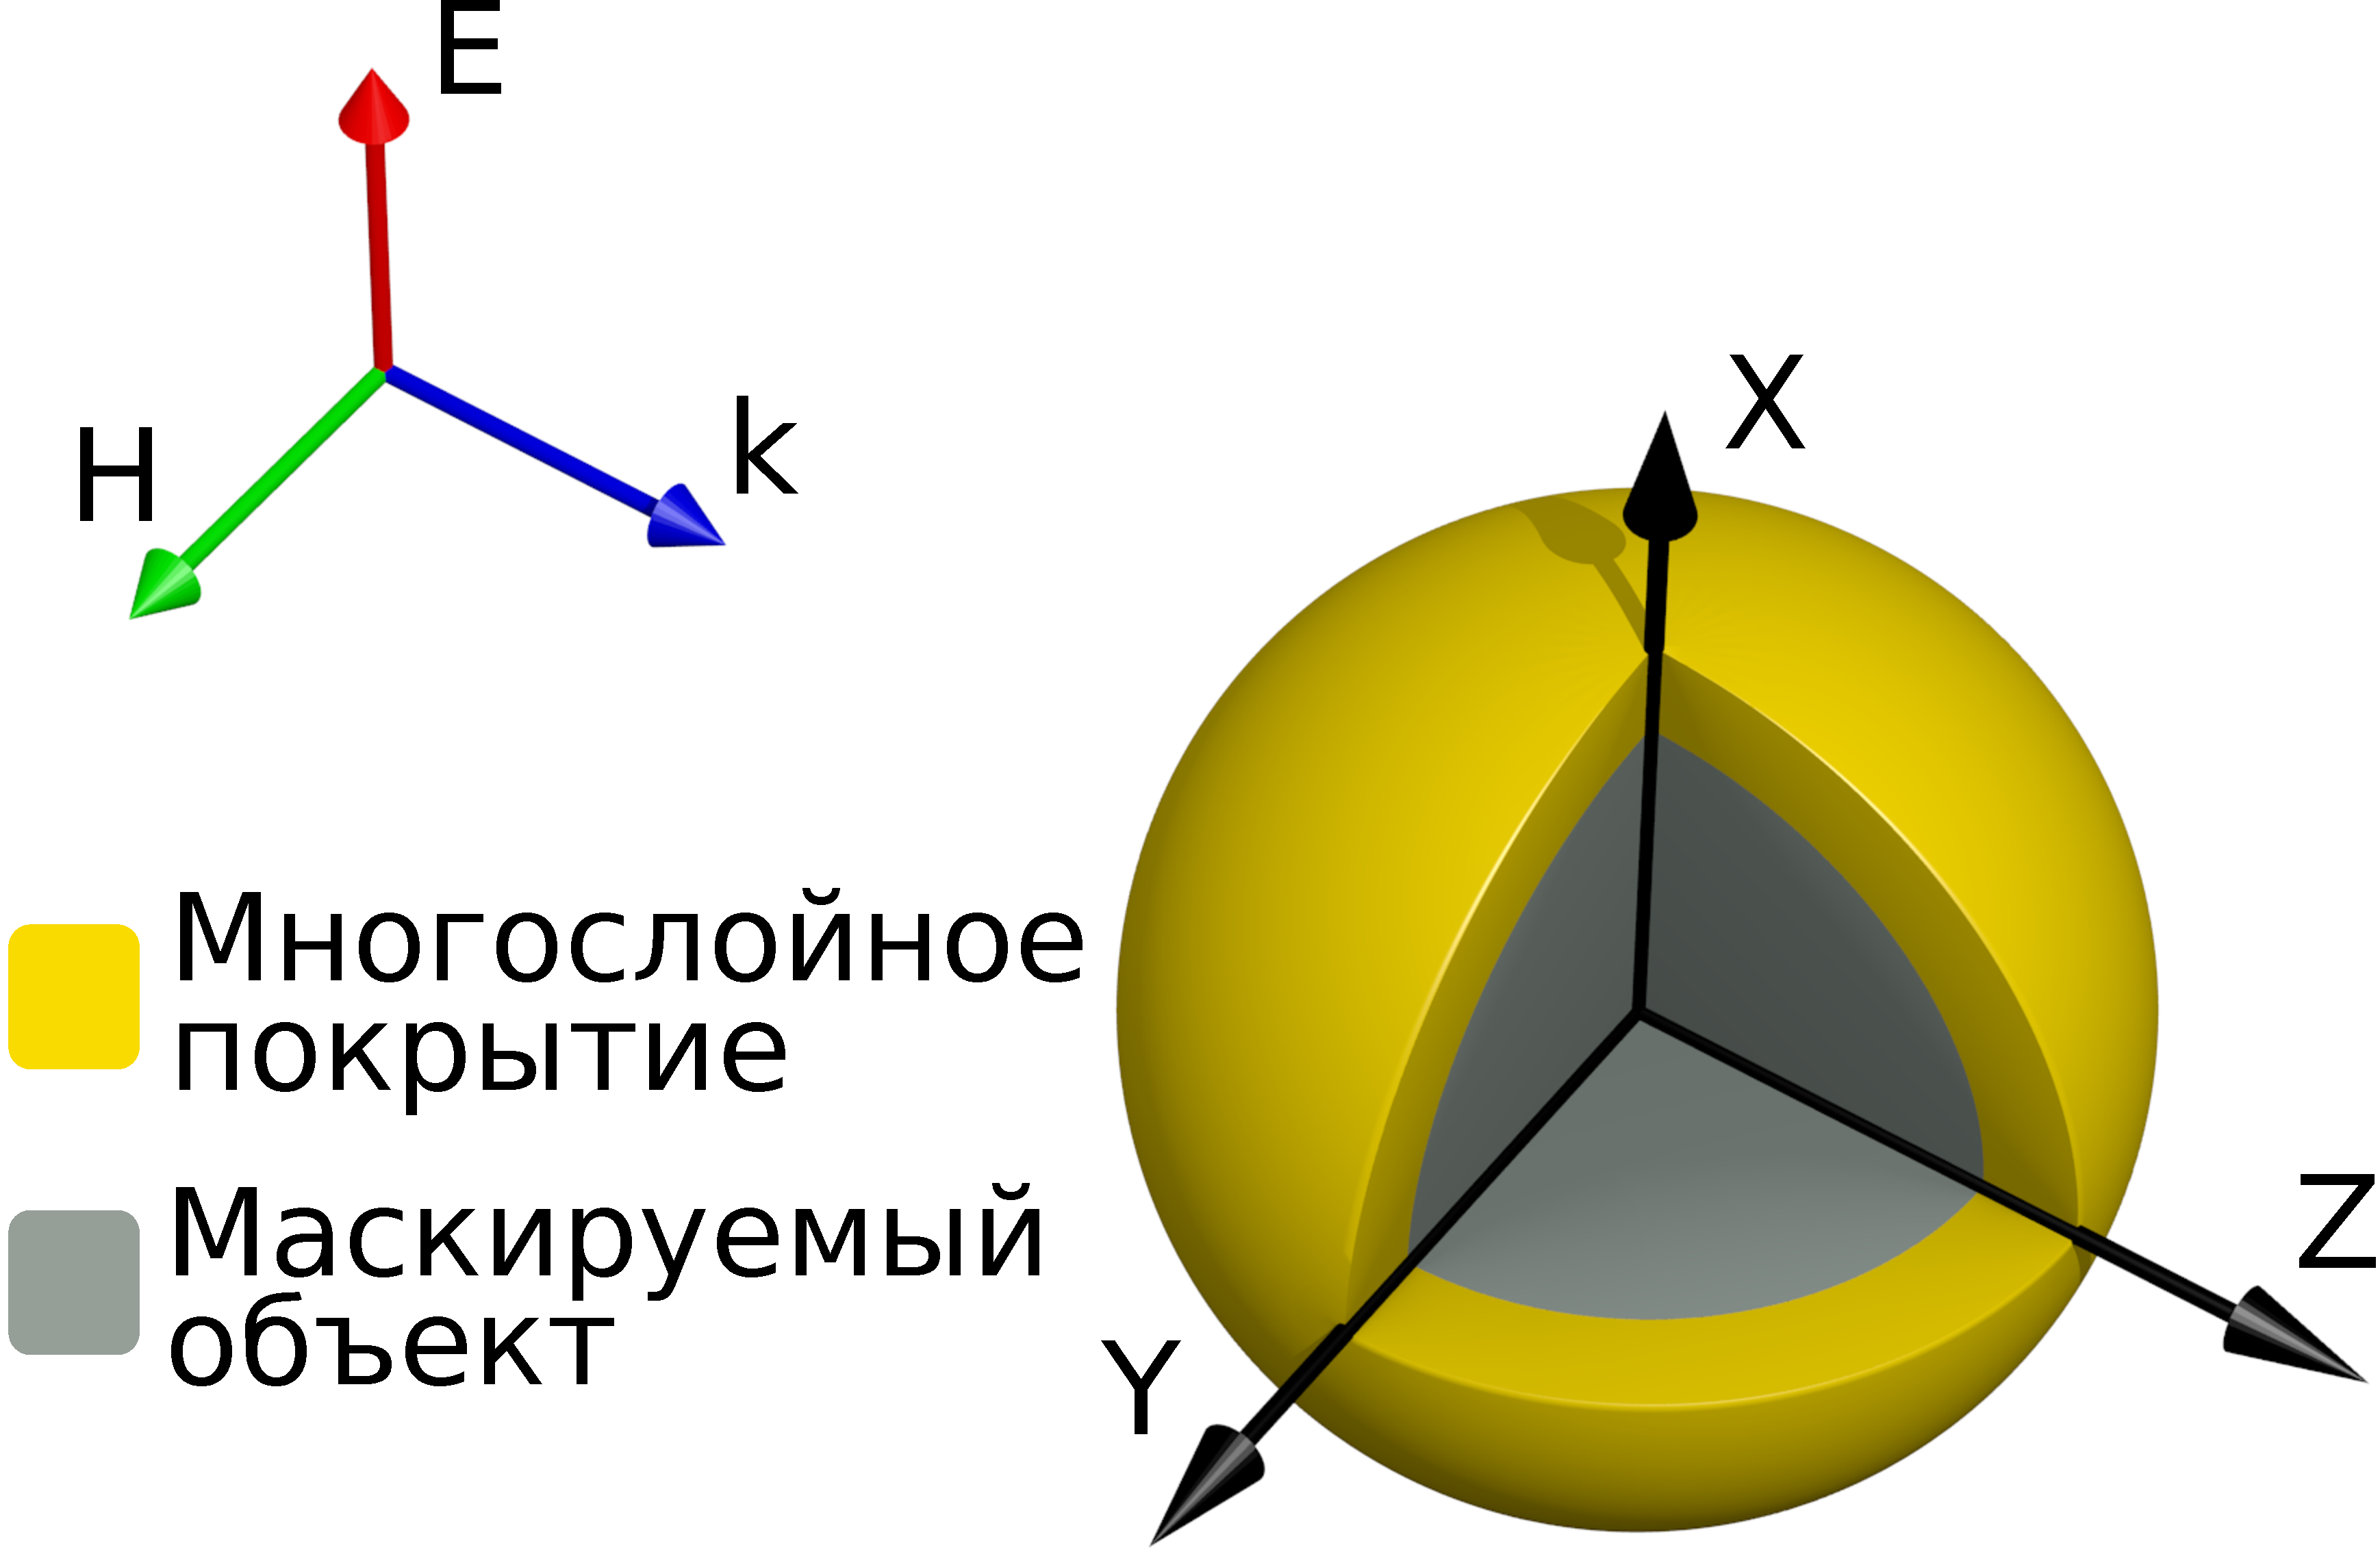
\includegraphics[width=0.57\linewidth]{model-view}}
  \end{minipage}\\
  \vfill
  \begin{minipage}[ht]{0.99\linewidth}
    \centering{а)}
  \end{minipage}\\
  \vfill
  \begin{minipage}[ht]{0.99\linewidth}
    \centering{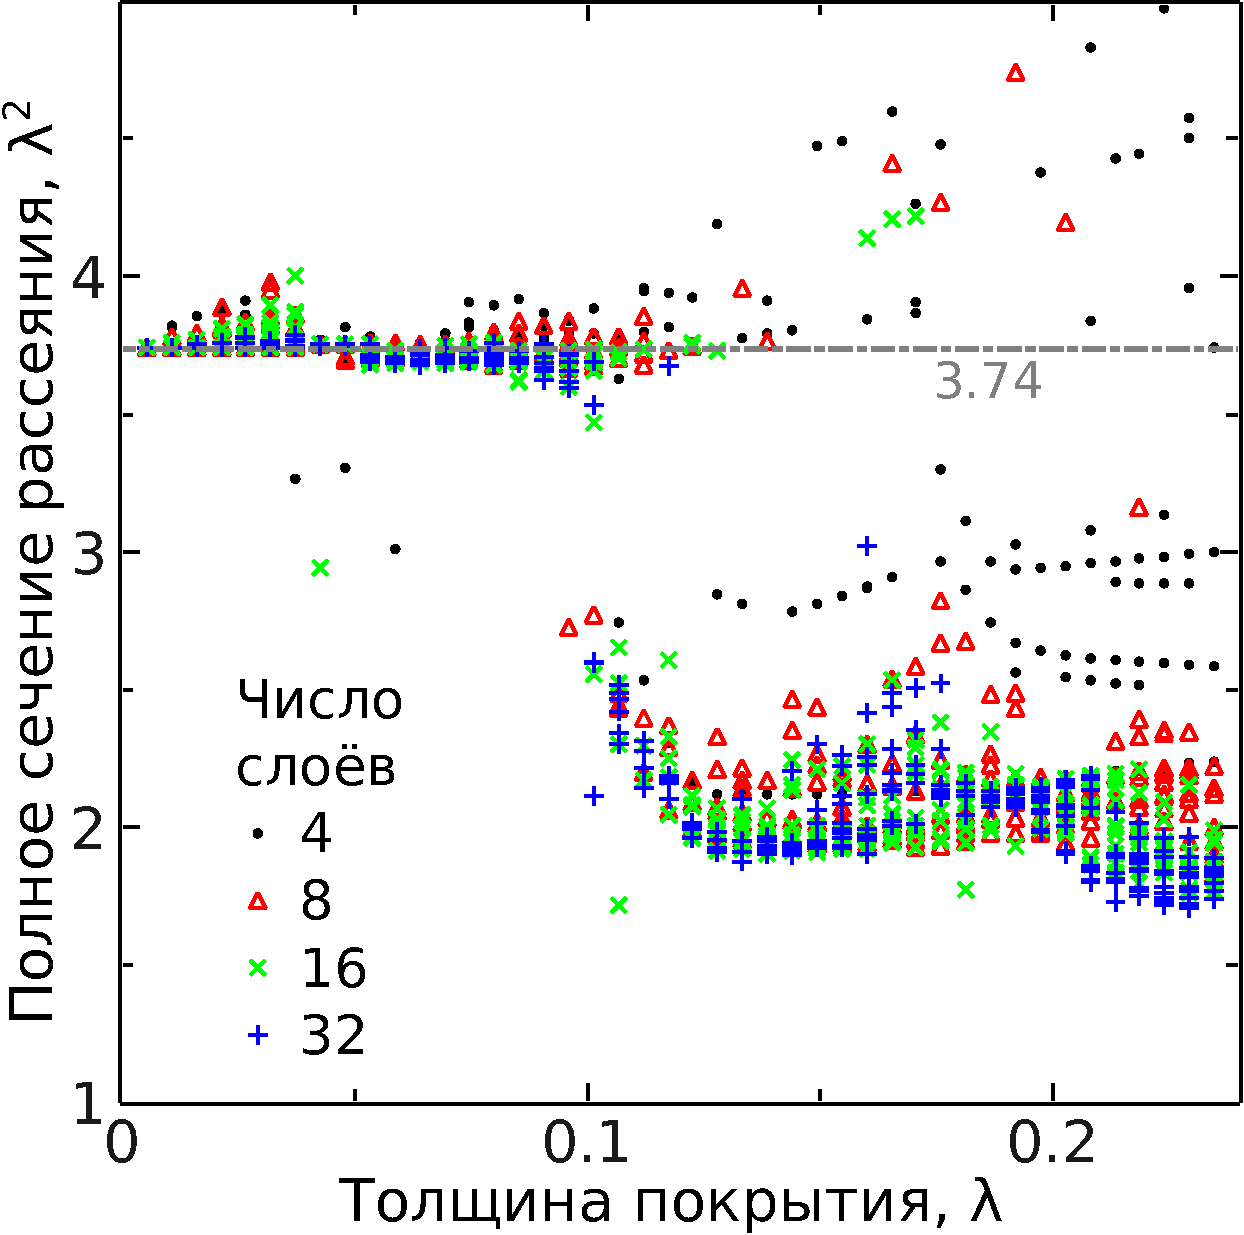
\includegraphics[width=0.57\linewidth]{rcs-overview}}
  \end{minipage}\\
  \vfill
  \begin{minipage}[ht]{0.99\linewidth}
    \centering{б)}
  \end{minipage}
  \vfill

  \caption{(a) Схематическое изображение изучаемой системы:
    маскируемый объект --- сфера из идеального проводящего материала
    внутри многослойного диэлектрического покрытия и падающая
    электромагнитная волна. (б)~Результат работы оптимизатора для
    объекта диаметром $1.5\lambda$.  Каждая отметка на графике
    соответствует одному дизайну покрытия, полученному в результате
    минимизации рассеяния. При толщине покрытия $>0.15\lambda$
    рассеяние можно уменьшить в $\sim 2$ раза.}
  \label{img:scattering}  
\end{figure}

\begin{figure}[p]
  \begin{minipage}[ht]{0.99\linewidth}
    \centering{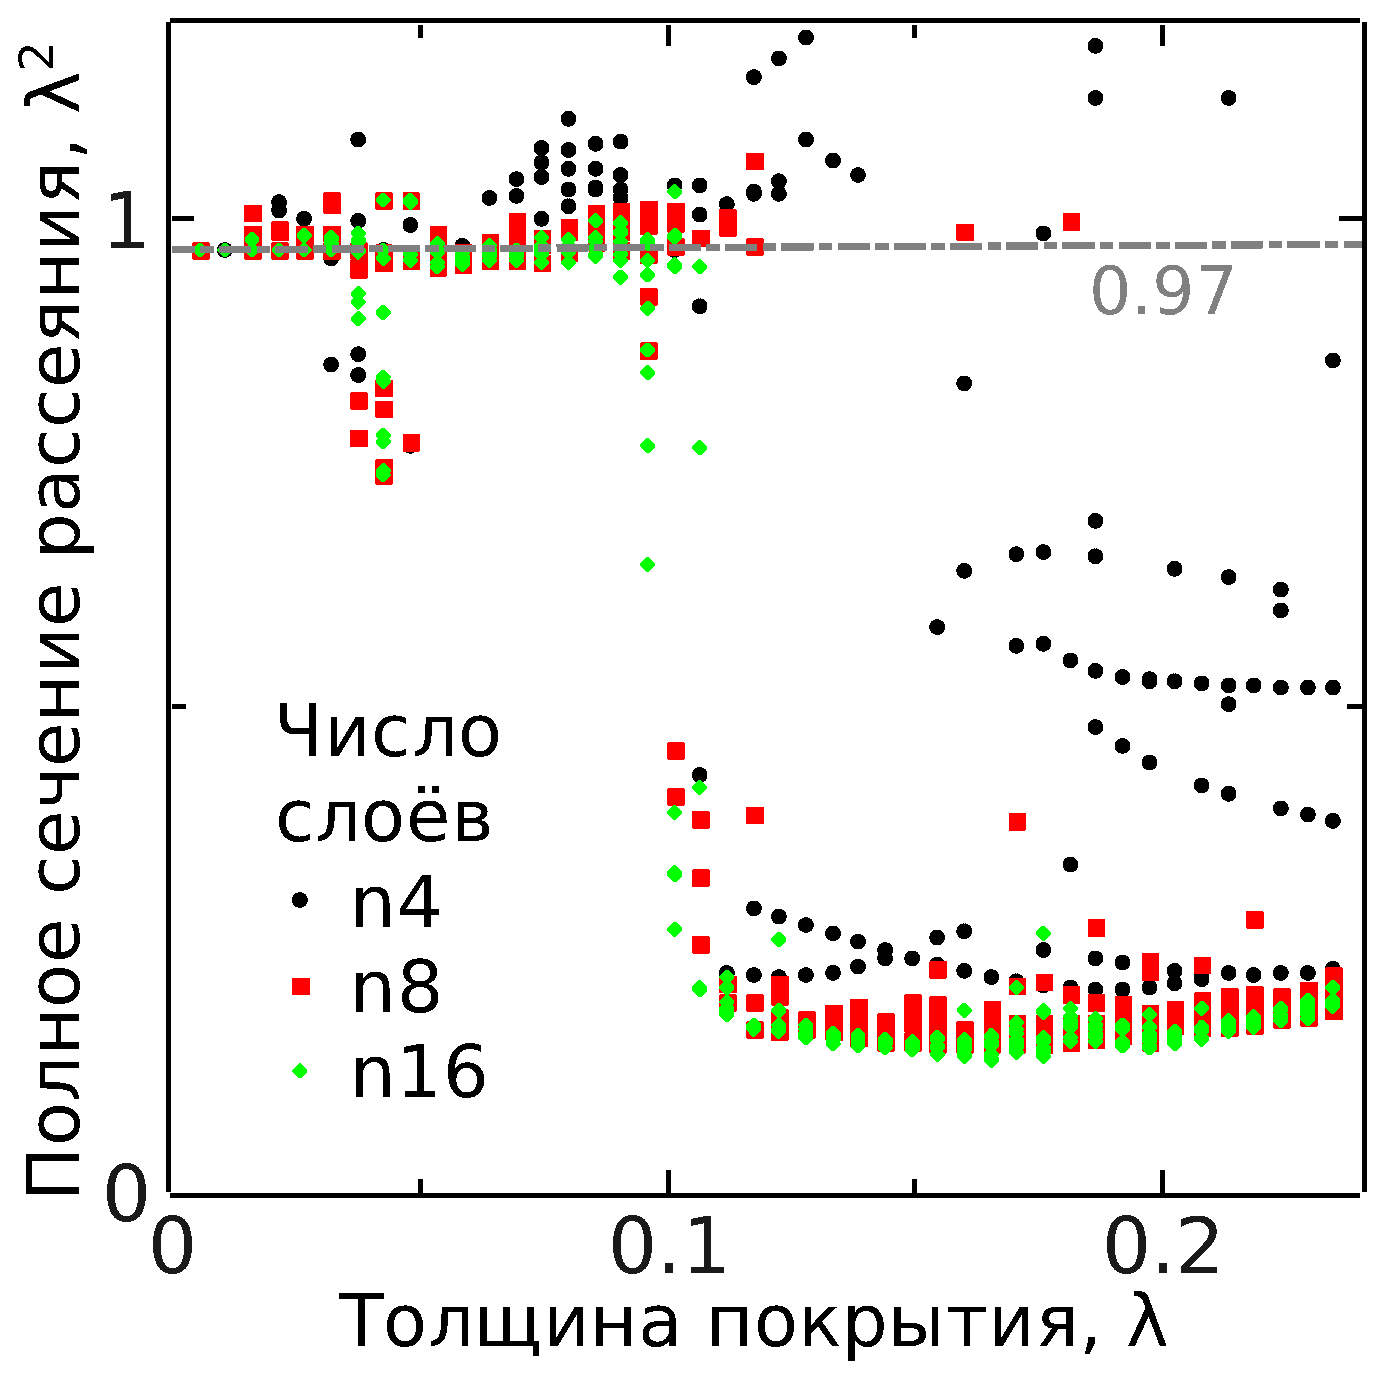
\includegraphics[width=0.57\linewidth]{rcs-overview-r14}}
  \end{minipage}\\
  \begin{minipage}[ht]{0.99\linewidth}
    \centering{а)}
  \end{minipage}\\
  \vfill
  \begin{minipage}[ht]{0.99\linewidth}
    \centering{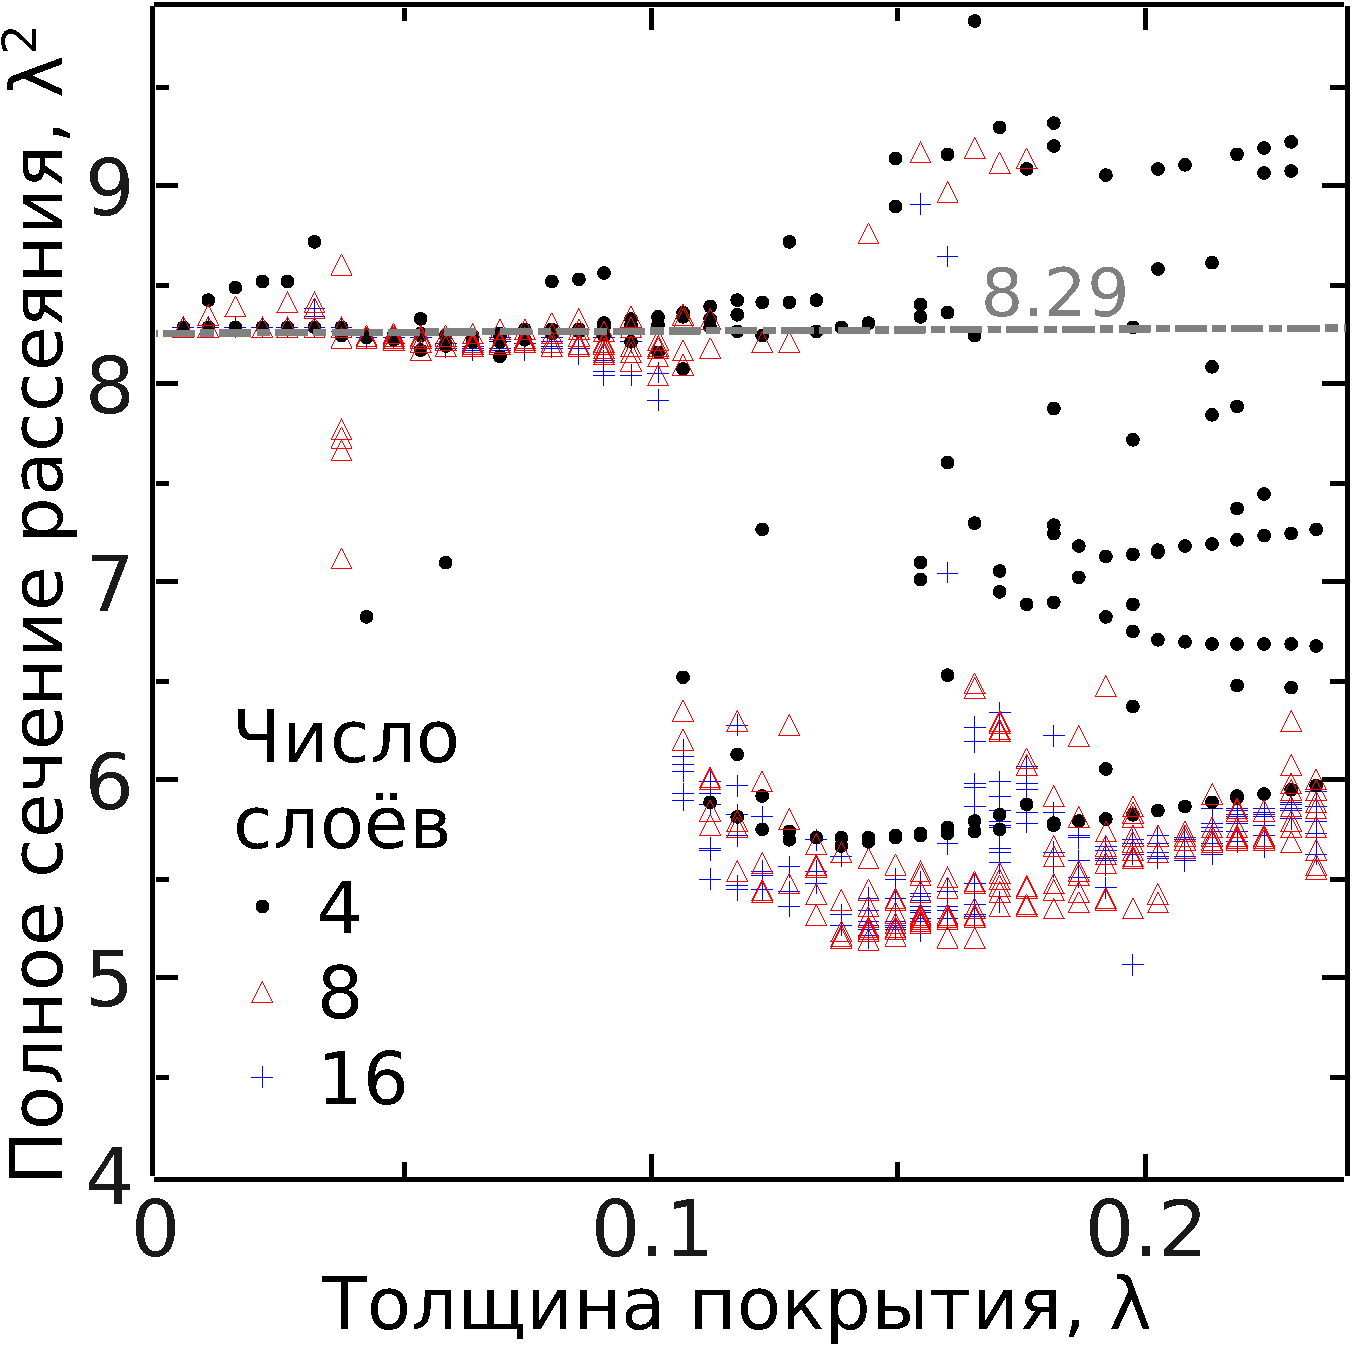
\includegraphics[width=0.57\linewidth]{rcs-overview-r42}}
  \end{minipage}\\
  \begin{minipage}[ht]{0.99\linewidth}
    \centering{б)}
  \end{minipage}
  \vfill
  \caption{Аналогично рисунку~\ref{img:scattering}(б), но для мишени
    (a)~${R_2 = 0.38\lambda}$ и (б)~${R_3 = 1.1\lambda}$.  Типичное
    значение уменьшения TSCS составило приблизительно -85\% и -35\%
    соответственно.  \label{img:rcs-overview-r14-42}}%
\end{figure}


Результат оптимизации в виде зависимости полного сечения рассеяния от
количества слоёв и общей толщины покрытия приводится на
рисунке~\ref{img:scattering}(б) и
рисунках~\ref{img:rcs-overview-r14-42}(а--б). Возможность снижения TSCS
была проверена в серии проходов оптимизации используя разные толщины
покрытия ${W < 0.24\lambda}$ с шагом $0.005\lambda$. Были
протестированы случаи разбиения покрытия на 4, 8, 16 (для всех
радиусов) и 32 слоя (для радиуса среднего размера). На рисунках хорошо
видно, что существует некоторое критическое значение
${W_c \approx 0.1\lambda}$ для общей толщины покрытия: дизайнов с
пониженной TSCS (относительно непокрытой мишени) для более тонких
покрытий практически нет. Большинство дизайнов с пониженной TSCS,
обнаруженных оптимизатором, имеют толщину покрытия больше
критической. Обсуждение небольшого количества дизайнов, приводящих к
заметному уменьшению TSCS и обладающих толщиной менее критической приводится на
странице~\pageref{ref:thin-designs}\label{backref:thin-designs}.


Рассмотрим более подробно случай радиуса мишени ${R_1 =
  0.75\lambda}$. Типичное снижение TSCS относительно непокрытой мишени
для толщины выше критической ${\Delta \approx -50\%}$ (в два раза
ниже). Непосредственно после превышения критической толщины
превалируют однодолинные дизайны~(рисунок~\ref{img:designs}(а), на
всех графиках дизайнов в настоящей работе мишень, представленная PEC
сферой, расположена слева, а открытое пространство справа).
\begin{figure}
  \hfill
  \begin{minipage}[ht]{0.44\linewidth}
    \centering{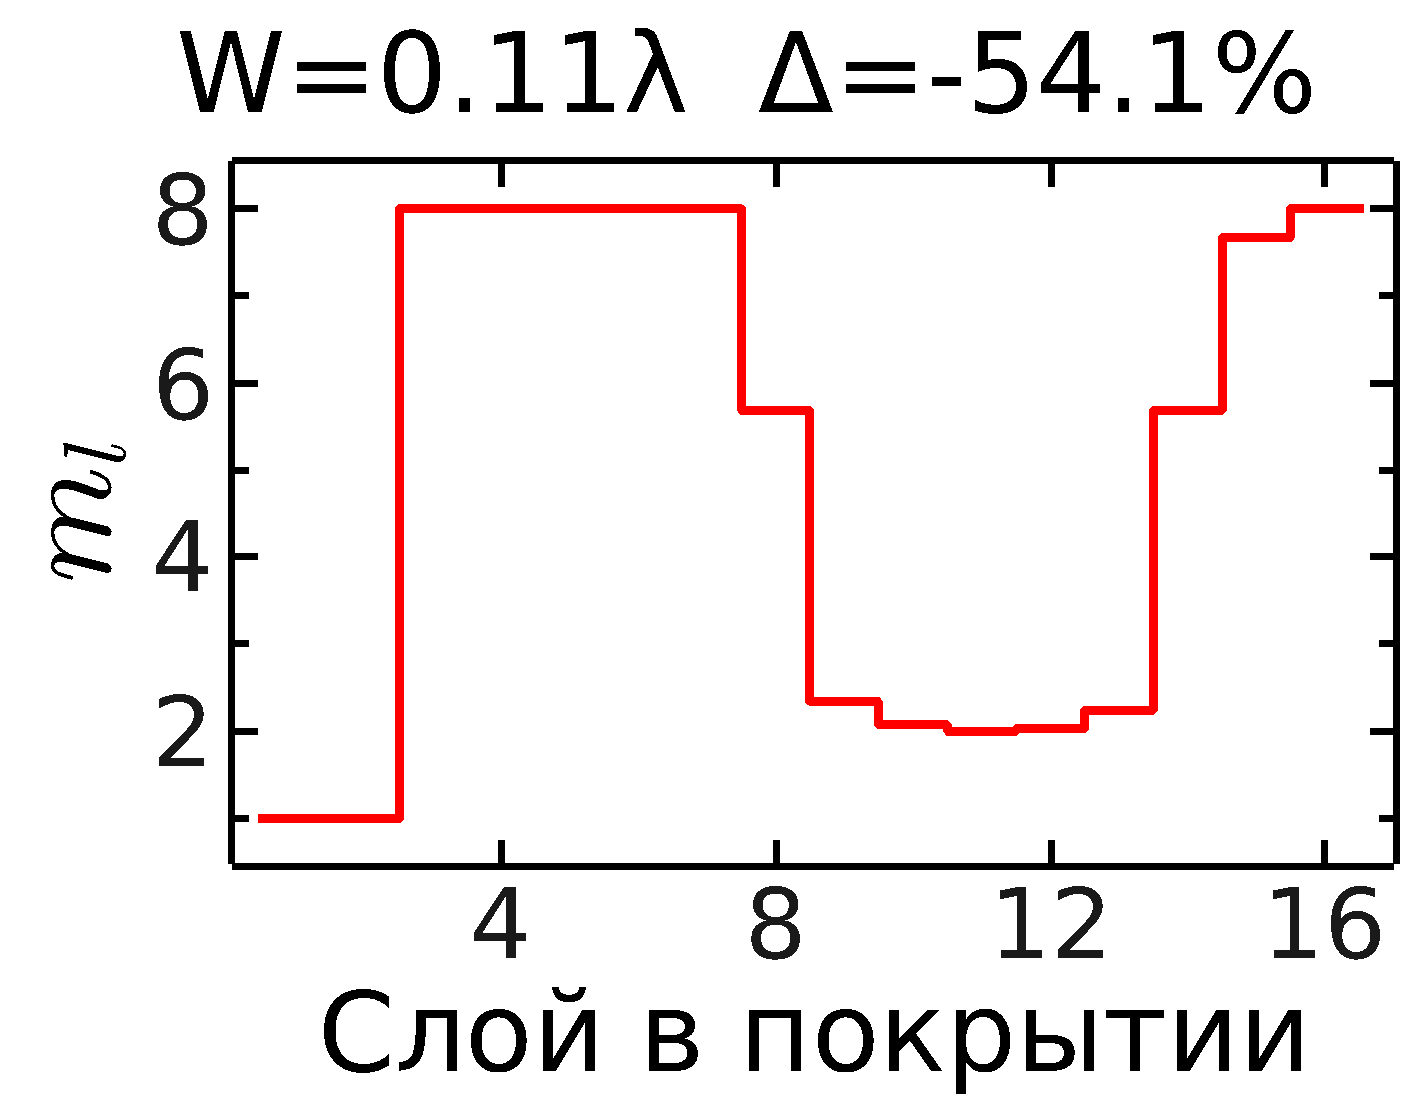
\includegraphics[width=0.95\linewidth]{w04-single-valley-index} \\ а)}
  \end{minipage}
  \hfill
  \begin{minipage}[ht]{0.44\linewidth}
    \centering{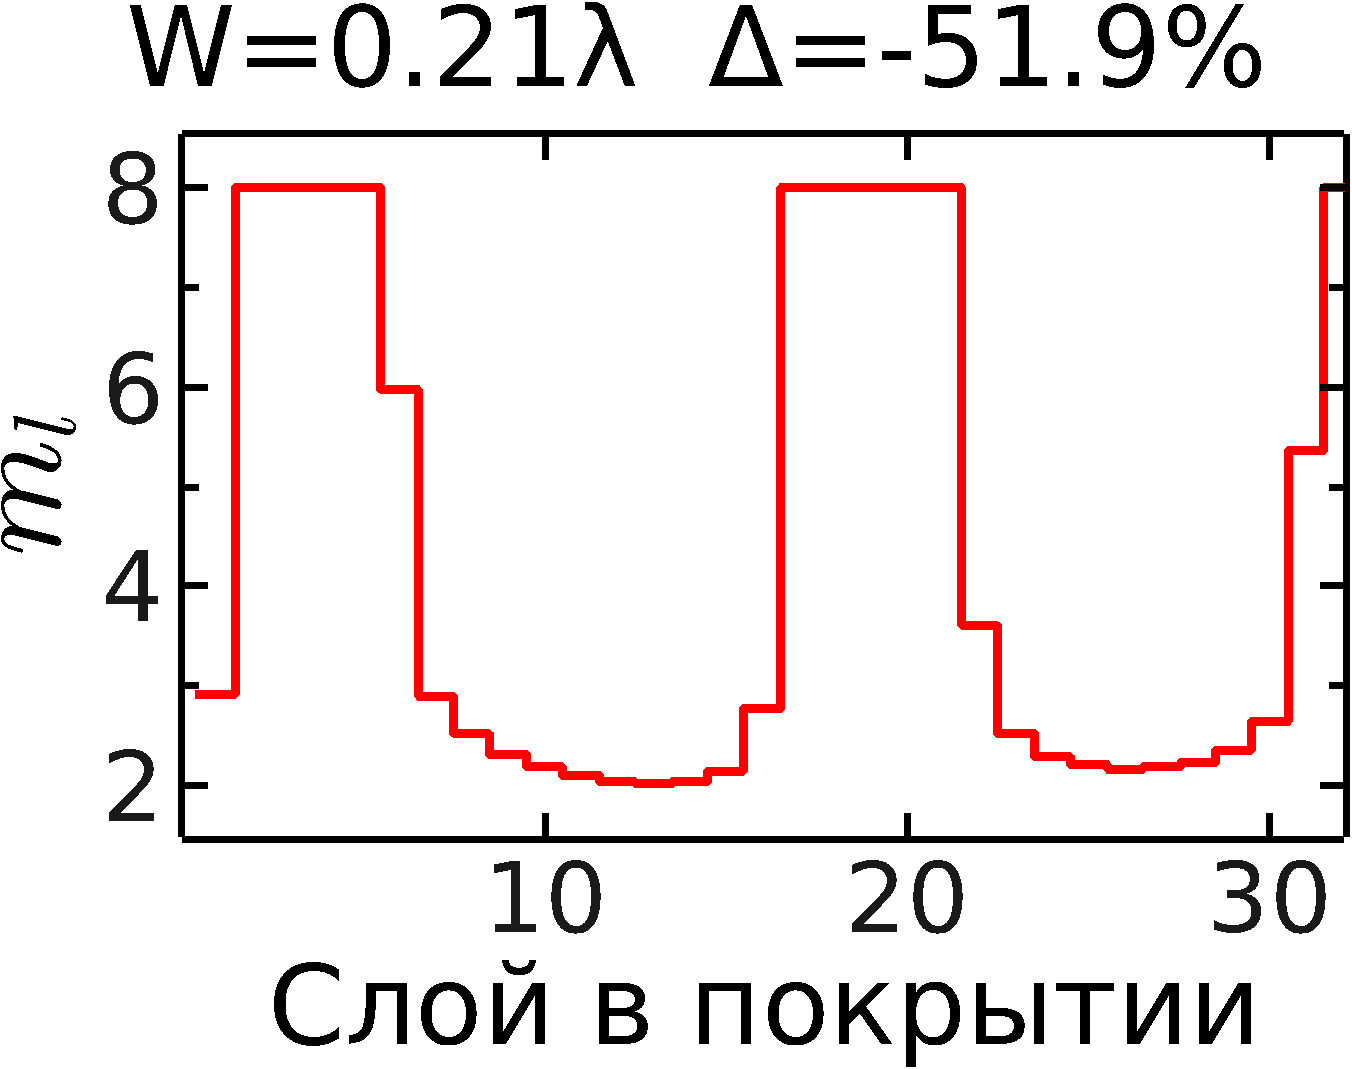
\includegraphics[width=0.95\linewidth]{w08-double-valley-index} \\ б)}
  \end{minipage}
  % \begin{minipage}[ht]{0.32\linewidth}
  %   \centering{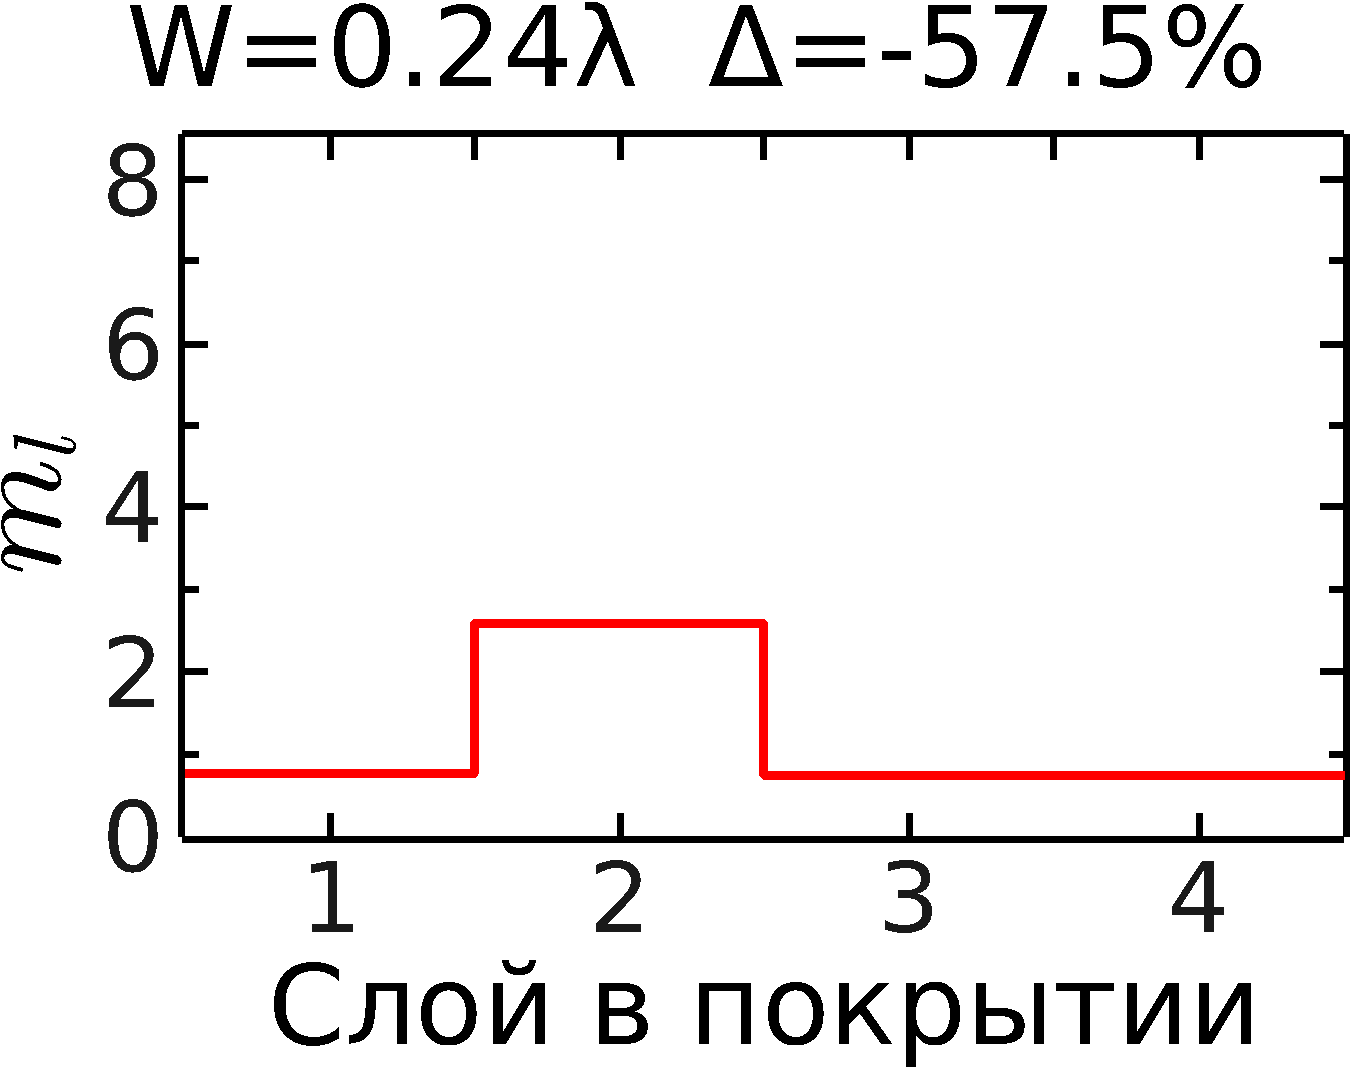
\includegraphics[width=0.95\linewidth]{index07-TO} \\ в)}
  % \end{minipage}
  \caption{Типичные дизайны, обеспечивающие наилучшую маскировку при
    толщине покрытия, равной (a)~$0.11\lambda$ и
    (б)~$0.21\lambda$. Максимальное значение показателя преломления
    было ограничено $n_{\mathrm{max}}=8$, а минимальное значение было
    равно $n_{\mathrm{min}}=1$ }
  \label{img:designs}  
\end{figure}
\begin{figure}[p]
  \begin{minipage}[h]{0.45\textwidth}
    \centering{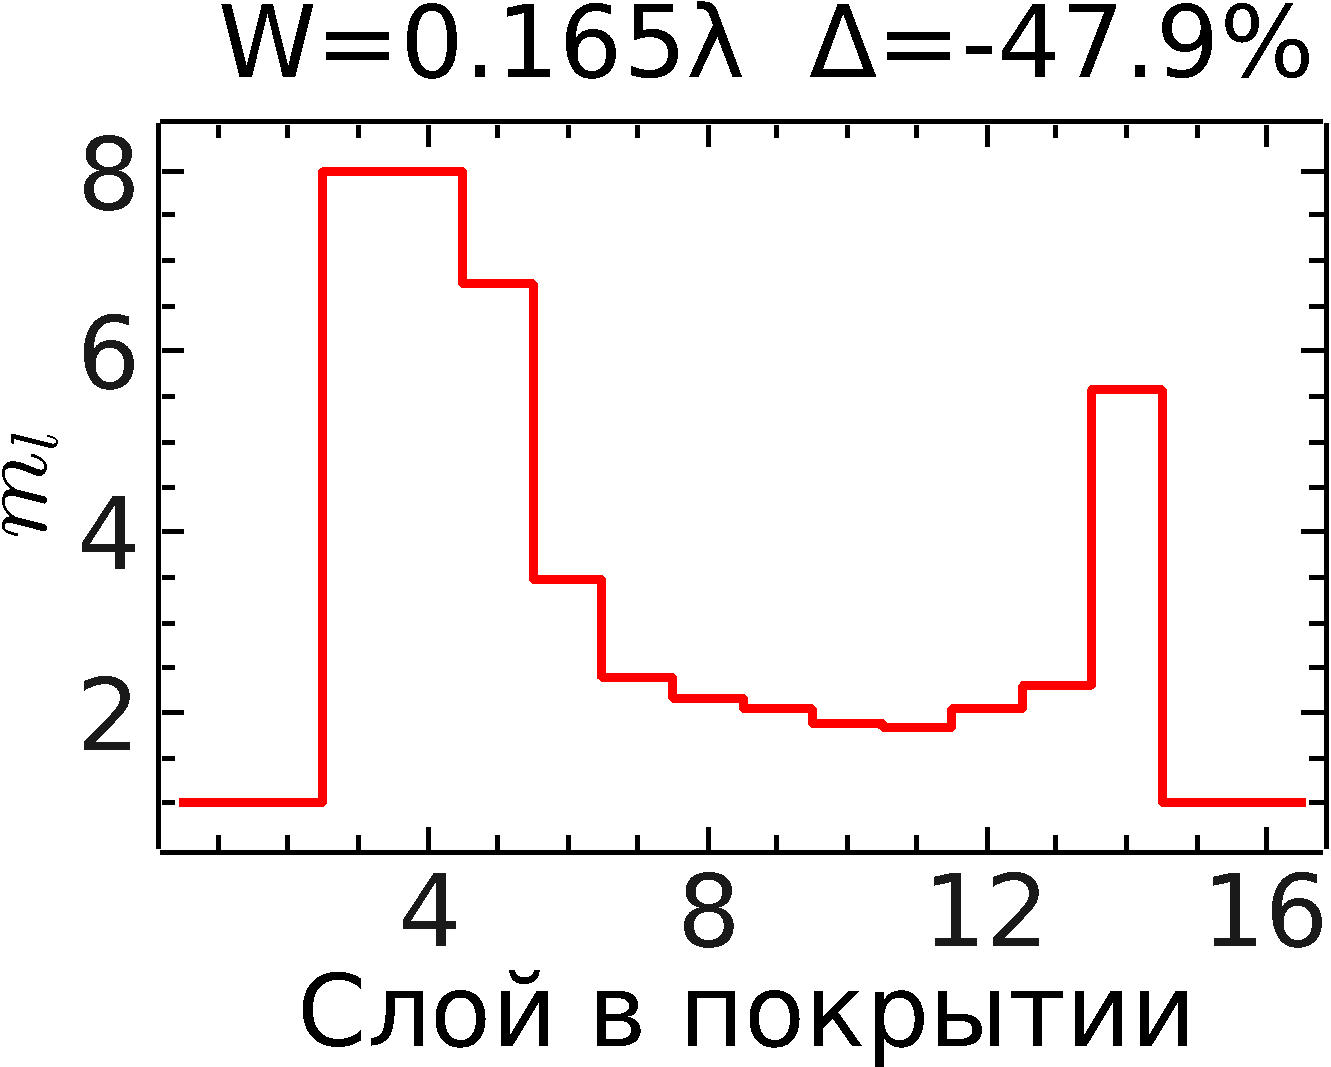
\includegraphics[width=0.99\textwidth]{w062-s-diff-479}\\а)}
  \end{minipage}
  \begin{minipage}[h]{0.45\textwidth}
    \centering{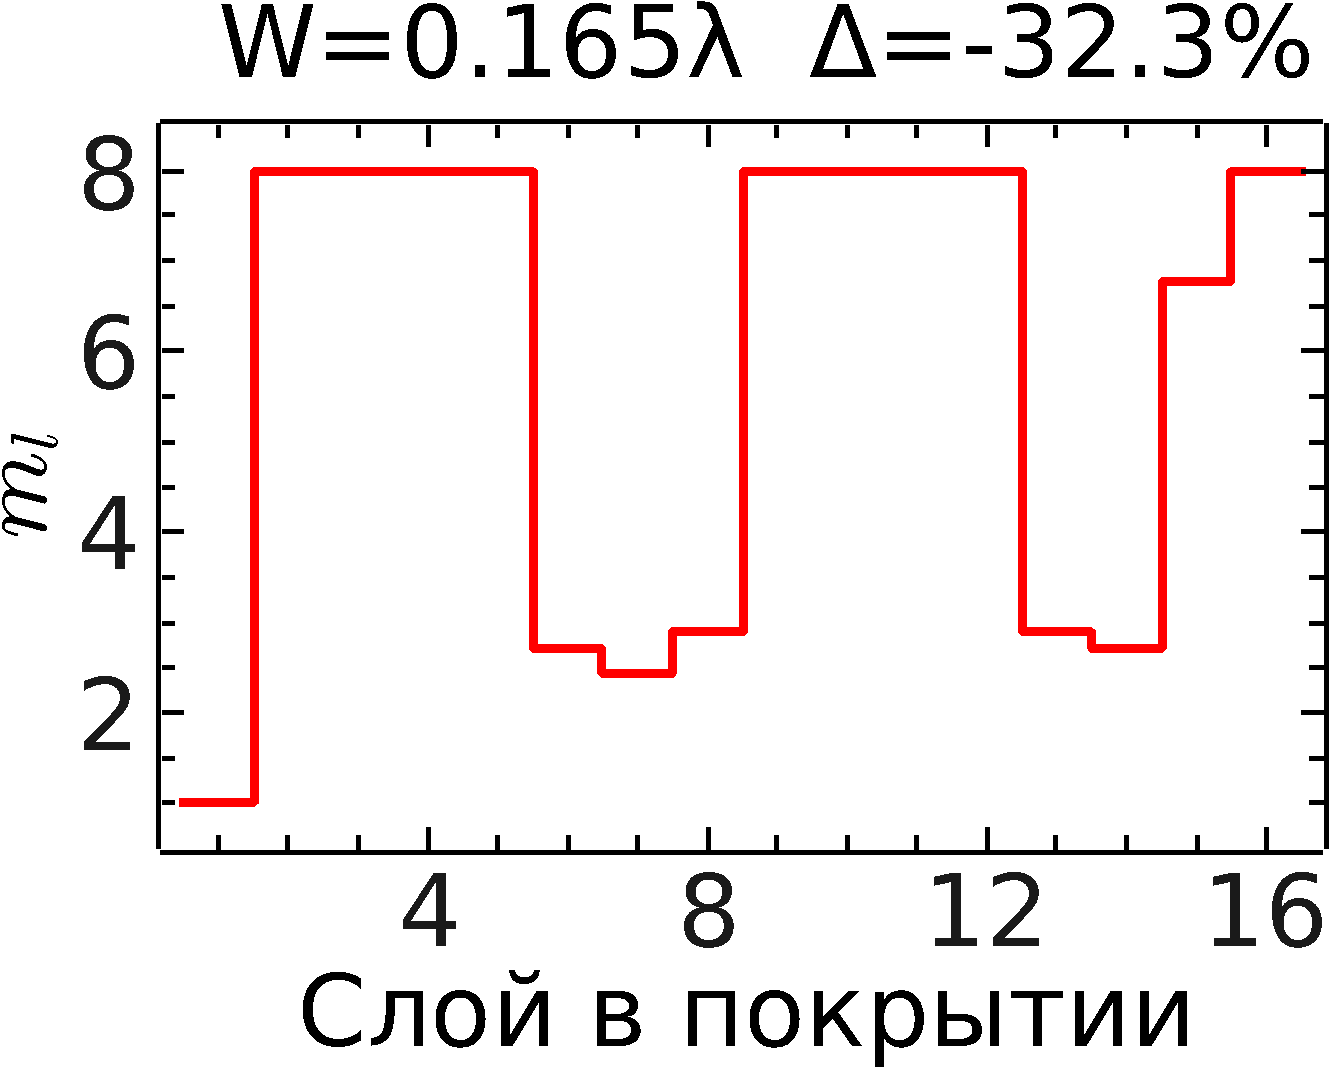
\includegraphics[width=0.99\textwidth]{w062-t-diff-323}\\б)}
  \end{minipage}\\
  \vspace{12pt}\\
  \begin{minipage}[h]{0.45\textwidth}
    \centering{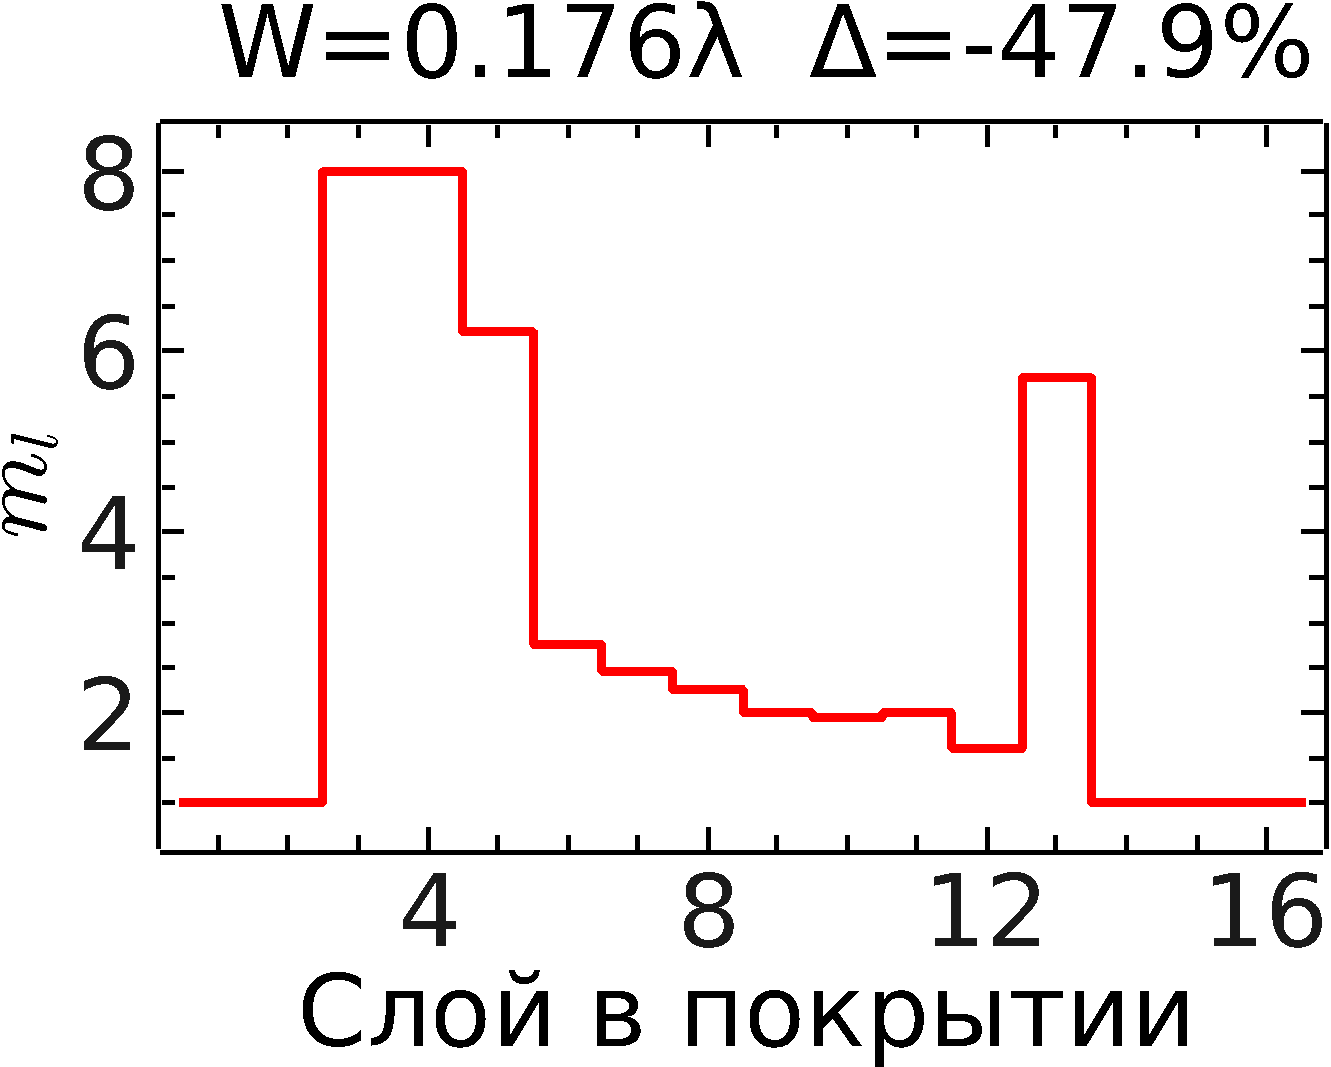
\includegraphics[width=0.99\textwidth]{w066-s-diff-479}\\в)}
  \end{minipage}
  \begin{minipage}[h]{0.45\textwidth}
    \centering{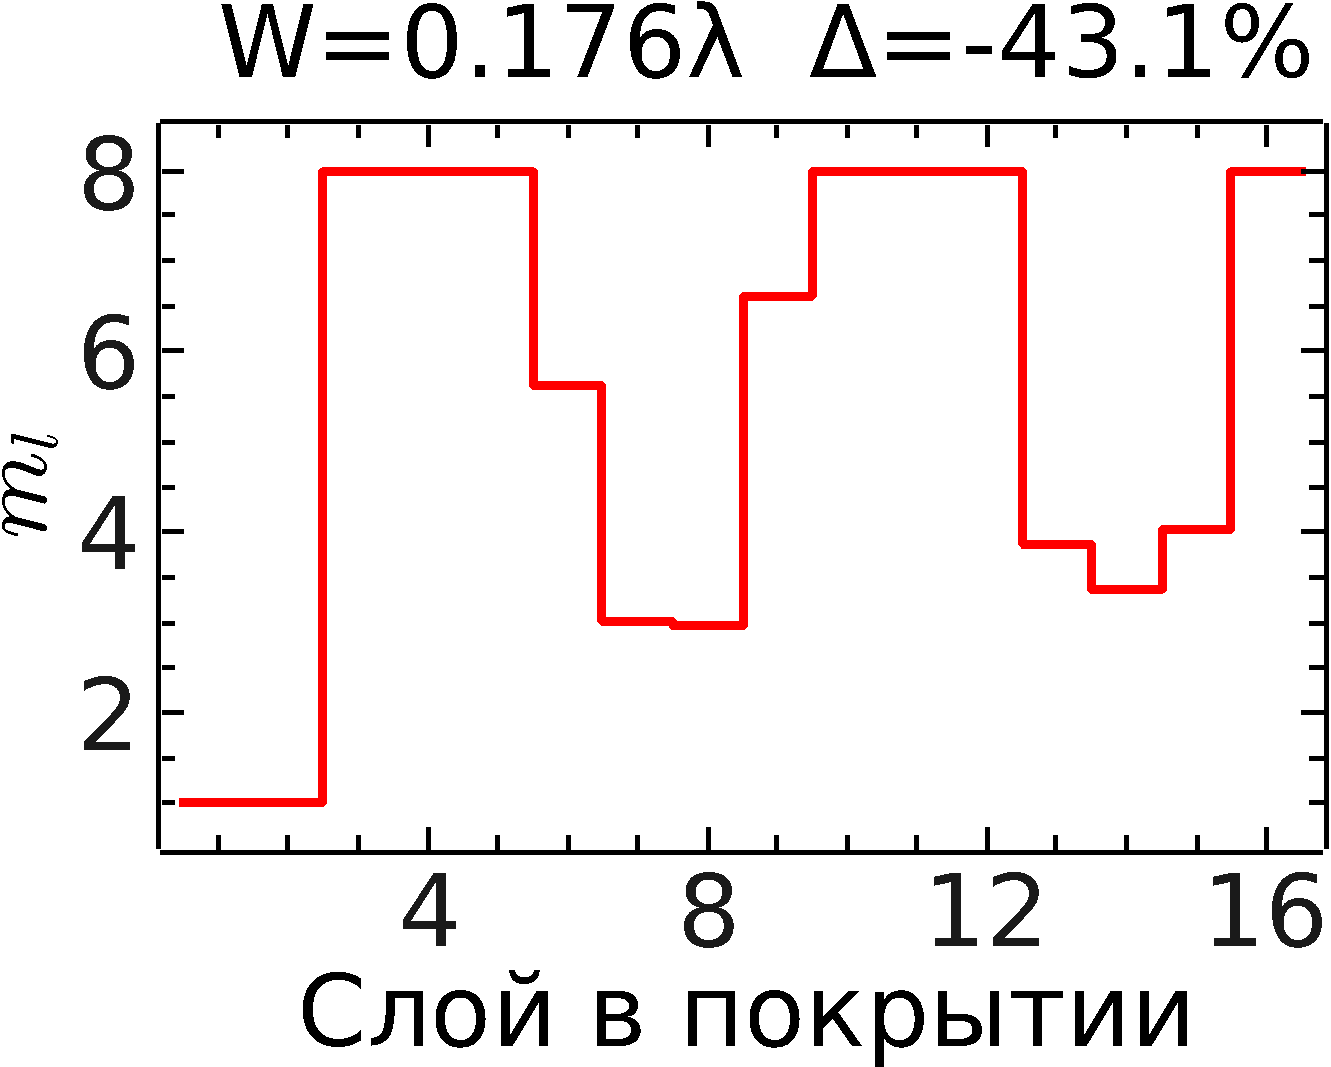
\includegraphics[width=0.99\textwidth]{w066-t-diff-431}\\г)}
  \end{minipage}\\
  \vspace{12pt}\\
  % \begin{minipage}[h]{0.45\textwidth}
  %   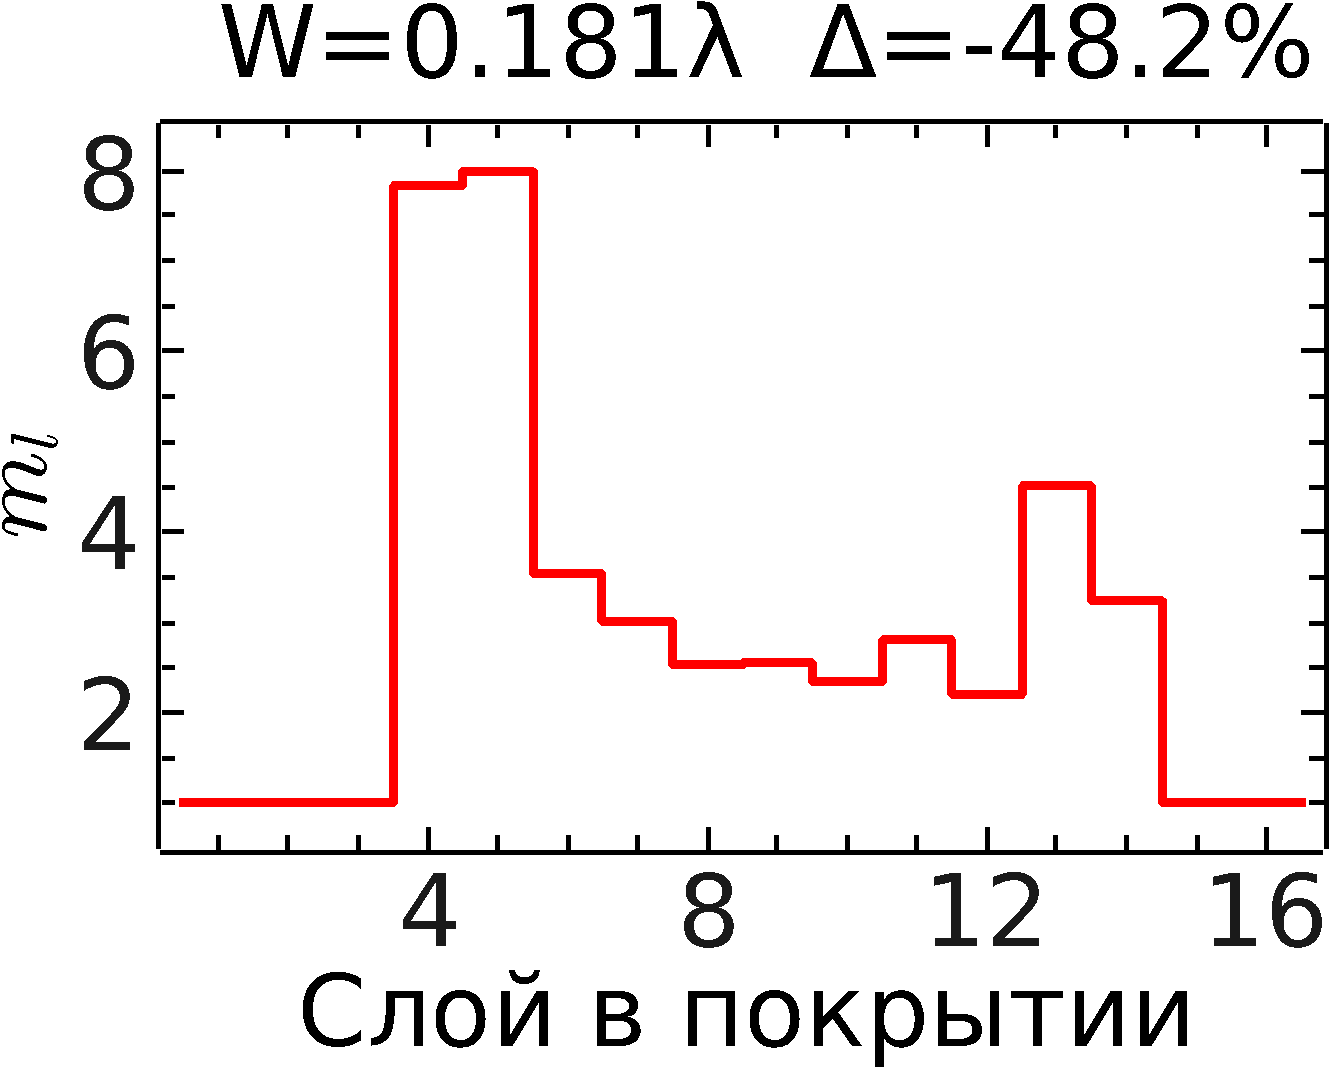
\includegraphics[width=0.99\textwidth]{w068-s-diff-482}
  % \end{minipage}
  % \begin{minipage}[h]{0.45\textwidth}
  %   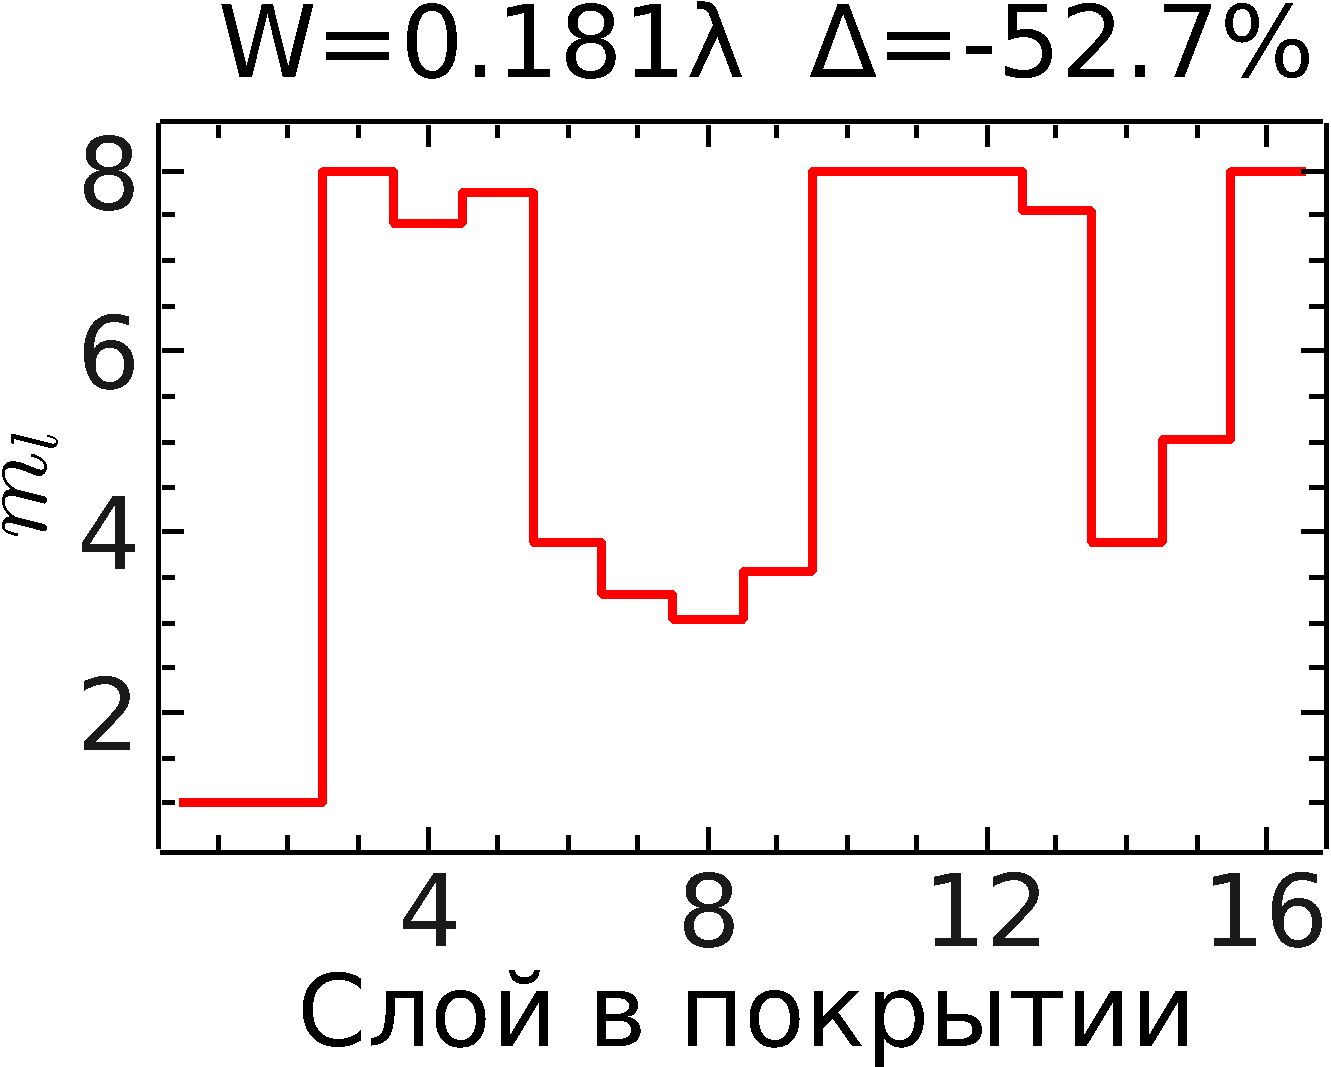
\includegraphics[width=0.99\textwidth]{w068-t-diff-527}
  % \end{minipage}\\
  % \vspace{12pt}\\
  \begin{minipage}[h]{0.45\textwidth}
    \centering{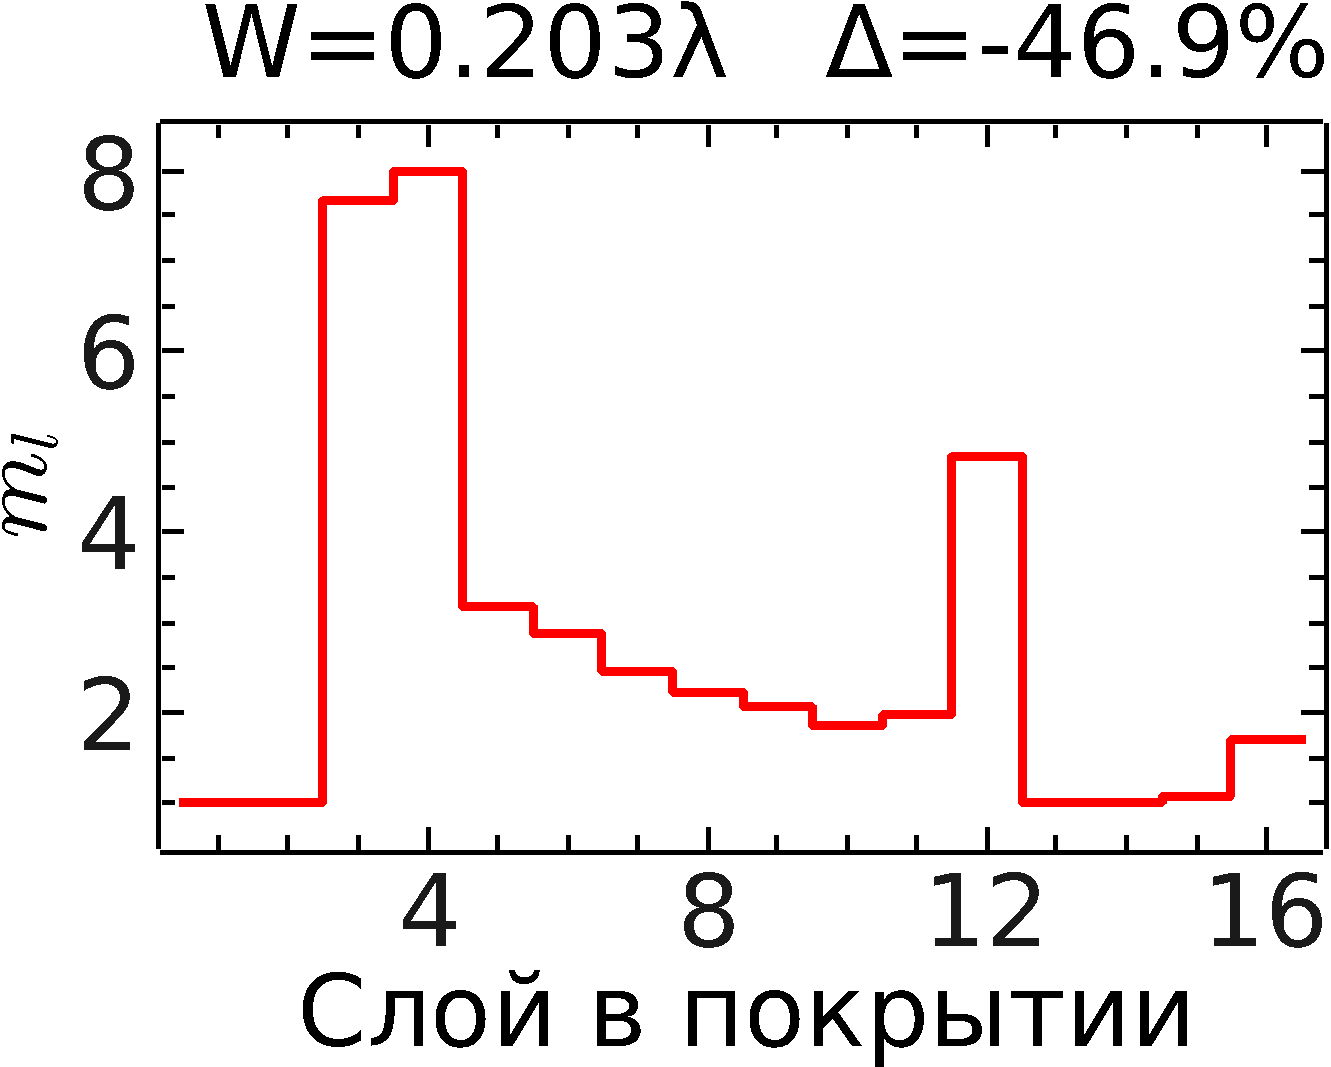
\includegraphics[width=0.99\textwidth]{w076-s-diff-469}\\д)}
  \end{minipage}
  \begin{minipage}[h]{0.45\textwidth}
    \centering{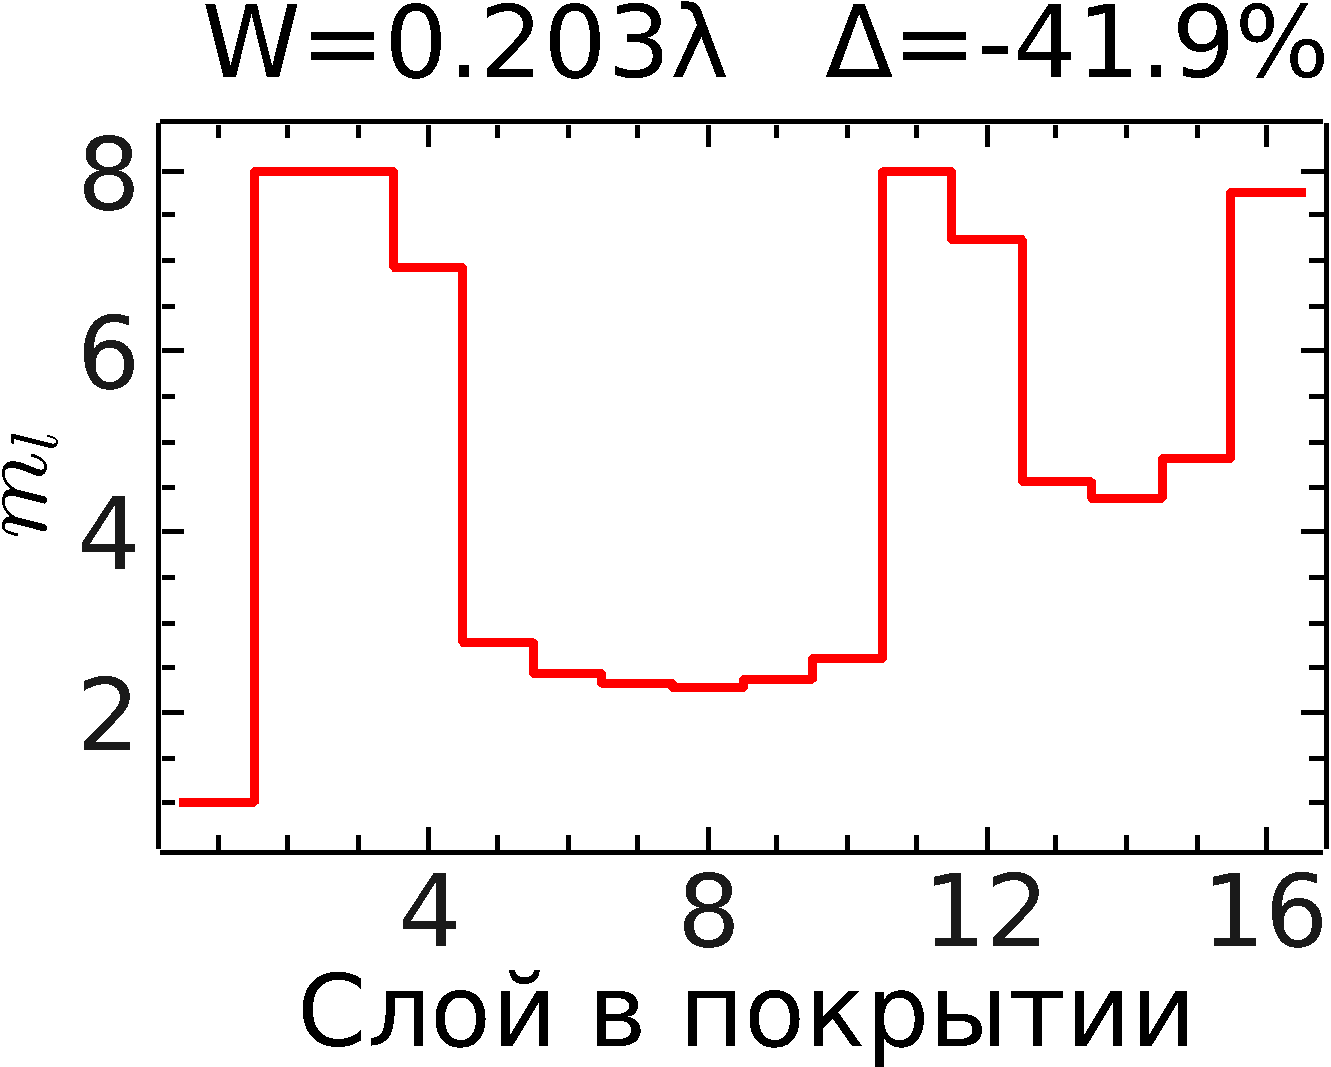
\includegraphics[width=0.99\textwidth]{w076-t-diff-419}\\е)}
  \end{minipage}%
  \caption{Переход от однодолинного к двухдолинному дизайну. Каждой
    паре (а--б), (в--г) и (д--е) соответствует одинаковая толщина
    покрытия. Каждый профиль показателя преломления был получен
    независимо, в отдельном проходе оптимизации.
    \label{img:transition}}%
\end{figure}
Такие дизайны, как правило, начинаются с воздушного промежутка между
покрытием и мишенью из PEC, затем следует быстрое увеличение
показателя преломления до максимально допустимого. После нескольких
слоёв с высоким значением величина показателя преломления постепенно
идёт вниз и снова вверх, образуя долину с низким значением внутри двух
стенок с высоким значением. Минимальное значение показателя
преломления в долине обычно не опускается ниже $m_l = 2$. За второй стенкой
долины величина показателя преломления резко падает с высокого значения до
уровня воздуха.


При росте толщины покрытия в диапазоне приблизительно от
${0.165\lambda}$ до ${0.205\lambda}$ происходит
переход~(рисунок~\ref{img:transition}) от
однодолинного~(рисунок~\ref{img:designs}а) к
двухдолинному~(рисунок~\ref{img:designs}б) дизайну. В этом диапазоне
независимые запуски оптимизатора могут выдавать то один, то другой вид
дизайна.  Для толщины покрытия более ${0.181\lambda}$ большинство
дизайнов имеет двухдолинную конфигурацию, немногие остальные не в
полной мере соответствуют однодолинной модели из-за наличия в покрытии
внутреннего или внешнего слоя с относительно высоким значением
показателя преломления. Для толщин, превышающих ${0.205\lambda}$,
однодолинных дизайнов обнаружено не было.

Во время перехода однодолинный дизайн выглядит довольно стабильным,
поскольку он достиг наилучшего состояния. Двухдолинный дизайн, видимо,
ограничен допустимой толщиной покрытия. С увеличением толщины покрытия
ширина его долин увеличивается. Ширина внутренней долины (которая
ближе к PEC мишени) растёт быстрее. Это может быть связано со
следующим фактом: электромагнитное поле в покрытии в основном
сосредоточено во внутренних слоях (см. рисунок~\ref{img:e32layer} и
раздел~\ref{sec:near-field}). Таким образом, дизайн внутренних слоёв
оказывает более сильное воздействие на итоговую TSCS по сравнению с
наружными слоями; следовательно, внутренние слои имеют приоритет при
оптимизации.

Существенного дополнительного снижения TSCS после перехода не
наблюдается. Можно предположить, что также возможны многодолинные
дизайны (с числом долин больше двух); однако их не удалось получить их
из-за ограничений по времени и по вычислительным мощностям. Была
проведена попытка оптимизации для толщины покрытия $0.64\lambda$, где
можно было ожидать наличия шести долин. Для этой толщины оптимизатор
смог найти некий дизайн~(рисунок~\ref{fig:thick}) с 54.3\% падением
TSCS.
\begin{figure}
  \centering{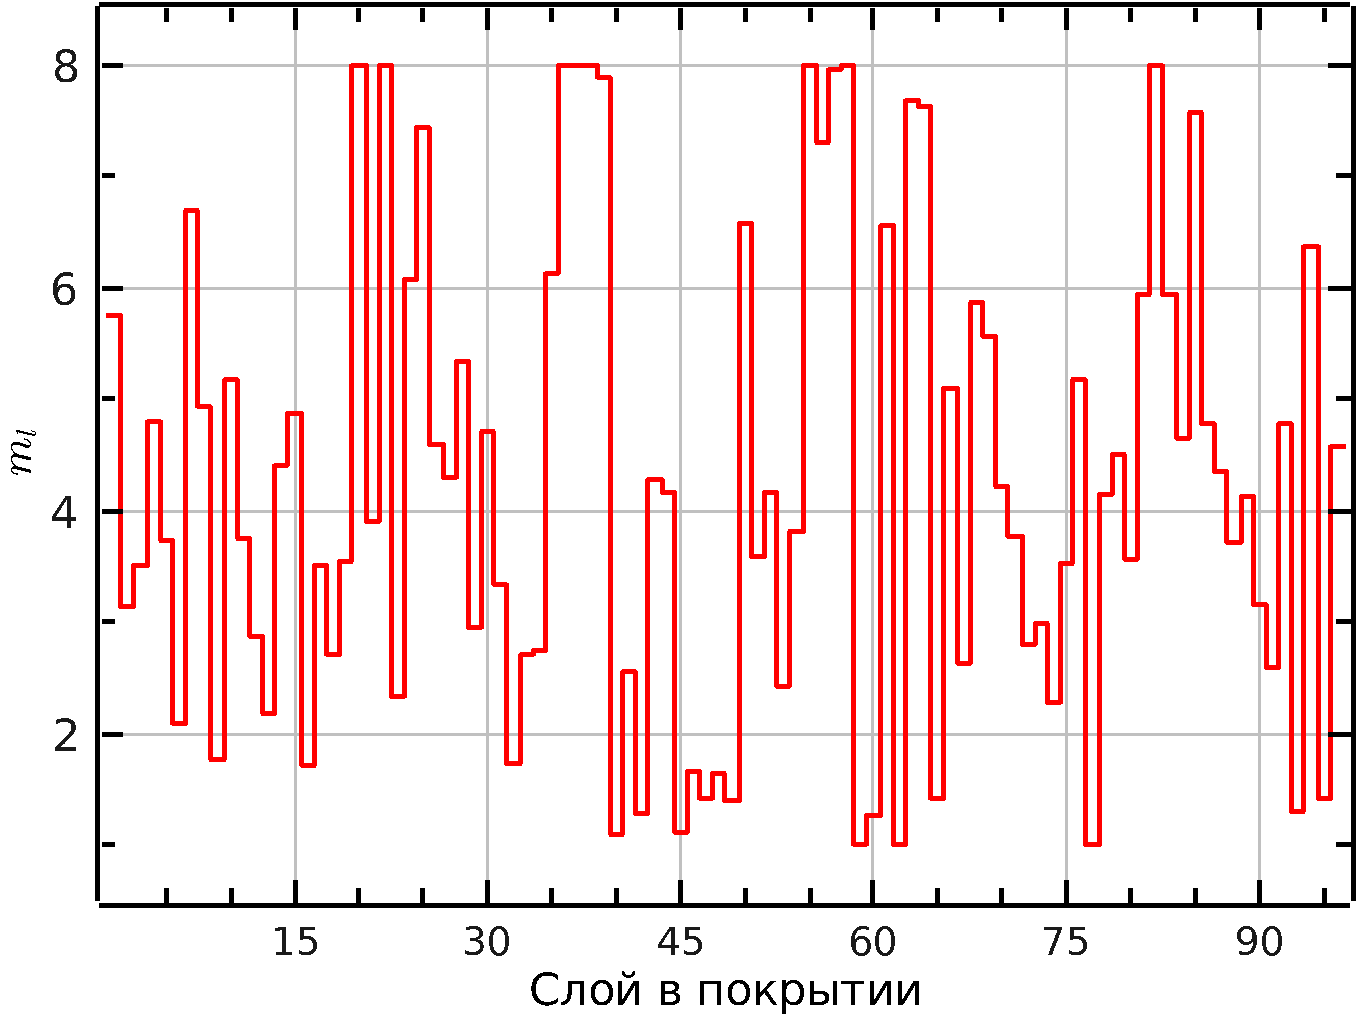
\includegraphics[width=0.87\textwidth]{w24-chaotic-index}}%
  \caption{Хаотический дизайн для толщины покрытия $W=0.64\lambda$
    $\Delta =-54.3$\% после 10~000 итераций оптимизации.
    \label{fig:thick}}%
\end{figure}
К сожалению, он выглядит довольно хаотично и не поддаётся простой
классификации, хотя и позволяет достичь значительного уменьшения
TSCS.

Необходимо отметить, что <<дёрганое>> поведение профиля показателя
преломления, хорошо видное в случае хаотического дизайна, может быть
частично обнаружено в случаях однодолинного и двухдолинных дизайнов,
описанных выше.  Это можно объяснить следующим образом: толщина
отдельного слоя внутри покрытия в десятки раз меньше длины волны (слои
являются субволновыми).  Таким образом, если поменять местами два
соседних слоя, то эффективное значение показателя преломления
поменяется слабо, как и величина падения TSCS.  В случае, если разница
в величине показателя преломления между этими слоями оказывается
достаточно большой, то будет наблюдаться <<дёрганое>> поведения
профиля показателя преломления, когда на общем среднем фоне большого
показателя преломления вблизи границы с долиной появляются одиночные
слои со значительно меньшим или большим значением показателя
преломления. Такую ситуацию стоит отличать от появление одиночного
проблемного слоя (напрмер, с большим показателем преломления
достаточно далеко от стенок долины, между ними), которое сразу приводит к
ухудшению маскирующих свойств покрытия, и легко поддаётся оптимизации.

В случае обмена местами двух соседних слоёв на границе долины это
может быть и не так. Предположим, что для дальнейшего улучшения
маскирующих свойств покрытия необходимо несколько сгладить границу
между долиной и её стенкой. В терминах эффективного значения
показателя преломления обмен соседних слоёв местами к этому и
приведёт. Эквивалентное решение, заключающееся в уменьшении большего
значения показателя преломления одного слоя и обратном действии для
второго слоя, может оказаться менее вероятным и зависит от формы
профиля.

Подобное поведение тонких многослойных покрытий представляет
существенную сложность для любого алгоритма оптимизации, так как очень
похожие друг на друга с физической точки зрения системы оказываются
сильно удалены друг от друга в многомерном пространстве входных
параметров.  Иначе говоря, у целевой функции, используемой в качестве
критерия оптимизации, наблюдаются многочисленные локальные минимумы
приблизительно равной амплитуды и формы, но разнесённые по разным
краям выбранного диапазона входных параметрах.  Этот факт при
использовании стохастического оптимизатора приводит к тому, что
конечный результат каждого прохода может отличаться от остальных
запусков оптимизации с теми же начальными параметрами.  По этой
причине для каждого набора входных параметров выполнялась серия
проходов оптимизации, а это, в свою очередь, обусловило наличие
нескольких отметок одного типа (с одинаковым количеством слоёв в
покрытии) для каждой исследованной толщины покрытия. Например, на
рисунках~\ref{img:scattering}(б) и~\ref{img:rcs-overview-r14-42}(а--б)
отметки с большим значением величины TSCS обычно обладают более
<<дёрганым>> профилем показателя преломления.

Несмотря на указанные сложности, адаптивный метод дифференциальной
эволюции воспроизводимо находит дизайны с уменьшенным рассеянием в
выбранном диапазоне толщин и числа слоёв в разбиении.  При
необходимости получения более гладких дизайнов несложно изменить
целевую функцию, например, домножив её на сумму абсолютных значений
разницы в показателях преломления всех смежных слоёв.  Можно
использовать и любую другую функцию, характеризующую локальную
неровность профиля, минимизируя <<дёрганность>> профиля одновременно
со значением TSCS.  На этом пути наиболее сложным может оказаться
поиск баланса между необходимостью получить наименьшее значение TSCS и
желанием получить более гладкий профиль показателя преломления.

Как следует из рисунка~\ref{img:scattering}, разбиения покрытия на
четыре слоя оказывается недостаточным для достижения оптимальных
значений TSCS.  Большинство дизайнов, обладающих TSCS более
$2.5\lambda^2$ и толщиной покрытия, превышающей критическую,
используют разбиение на 4 слоя.  Этот результат хорошо понятен:
четырёх слоёв недостаточно, чтобы с одной стороны задать оптимальную
эффективную ширину долины, а с другой стороны максимально использовать
доступный диапазон значений для показателя преломления.  При этом
разбиения на 8 слоёв оказывается достаточным для того, чтобы получить
результаты, сравнимые со случаями 16 и 32 слоёв (особенно для
диапазона толщин покрытия, соответствующих однодолинному дизайну).
Тем не менее, у разбиения на 32 слоя есть небольшое преимущество в
случае большой толщины покрытия (${> 0.21\lambda}$). Объяснение этого
факта по сути аналогично случаю четырёх слоёв, однако здесь, скорее
всего, большее значение оказывает необходимость в большем числе слоёв
для оптимального описания формы профиля между областями с большим и
меньшим значениями показателя преломления.
\begin{figure}
  \centering{
    % Use pdfcrop to remove white margins
    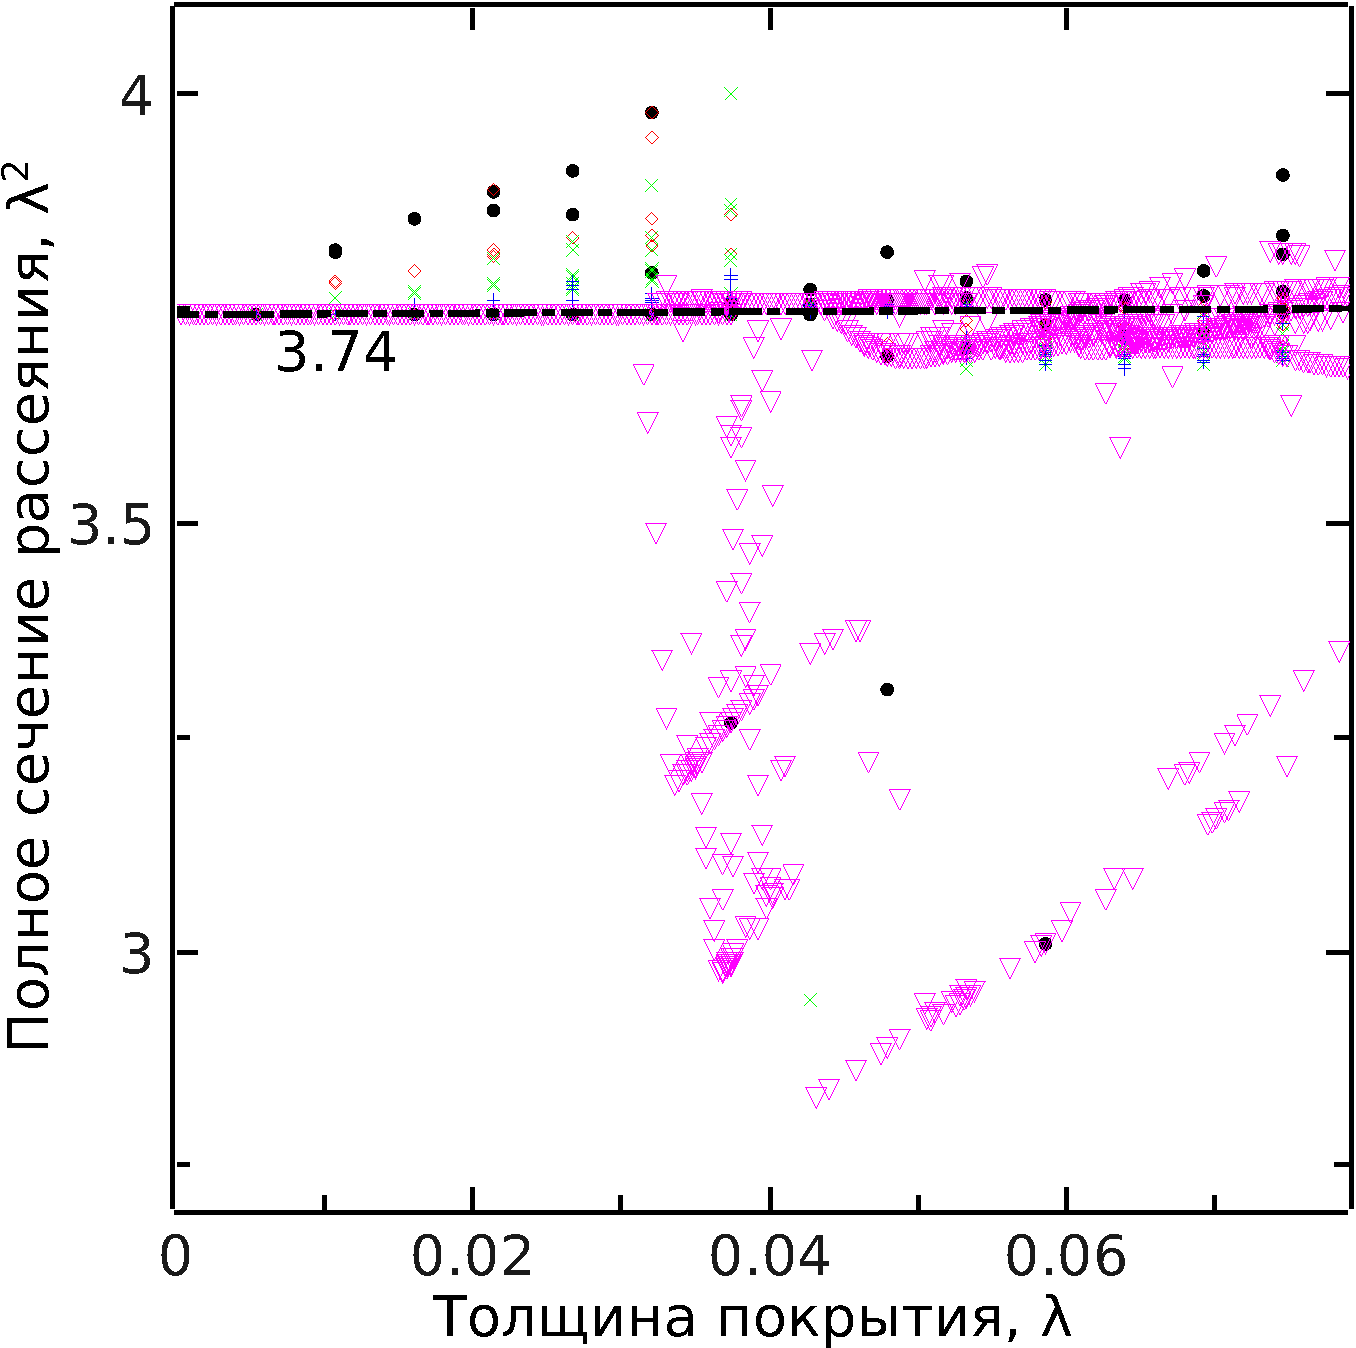
\includegraphics[width=0.67\textwidth]{rcs-overview-thin}%
      \caption{Увеличенная часть рисунка~\ref{img:scattering}(б) с
        дополнительными результатами оптимизации (треугольники без
        заполнения) для случая толщины покрытия меньше критической.
        Каждая отметка обозначает конечный результат одного прохода оптимизации.
        \label{img:rcs-overview-thin}}%
  }
\end{figure}

Как было указано ранее на
странице~\pageref{backref:thin-designs}~\label{ref:thin-designs}, при
проведении оптимизации было обнаружено небольшое число дизайнов с
маскирующим эффектом в случае толщины покрытия значительно меньше
критической.  Чтобы изучить такие дизайны мы провели дополнительную
серию оптимизаций (треугольники без заполнения на
рисунке~\ref{img:rcs-overview-thin}).  Основываясь на ранее полученных
результатах (а также по причине ограниченных вычислительных ресурсов),
мы использовали разбиение только на 4 и 8 слоёв.  Для того чтобы
добиться воспроизводимости результатов, нам пришлось уменьшить шаг
сканирования для толщины покрытия и увеличить размер популяции в
настройках оптимизатора.  Несмотря на это, всего лишь 218 проходов
оптимизации из $\sim$4~000 смогли достичь значения TSCS менее
$3.6\lambda^2$.  Лучший дизайн достиг $\Delta = -24\%$ падения TSCS для толщины
покрытия $W=0.043\lambda$.  Аналогичные дизайны для сверхтонких
покрытий, полученные в разных независимых прогонах оптимизации,
образуют хорошо различимые зависимости при изменении толщины на
рисунке~\ref{img:rcs-overview-thin}.  Физический принцип, определяющий
возникновение маскирующего эффекта в таких покрытиях, остался не до
конца понятым и в случае необходимости он может быть дополнительно
изучен в продолжении настоящей работы.


\section{Зависимость от показателя преломления}

Свойства сферического маскирующего покрытия, состоящего из нескольких
слоёв одинаковой толщины, задаются рядом параметров. В предыдущем
разделе были рассмотрены возможности для уменьшения TSCS в зависимости
от общей толщины покрытия, числа слоёв, размера мишени. Последним
параметром, определяющим результат оптимизации, является диапазон, в
котором может изменяться показатель преломления каждого слоя.  Для
вышеизложенных результатов компьютерного моделирования он был
ограничен интервалом от одного (воздух) до $8$.  Такой выбор позволил
соотнести получаемые результаты с работой~\cite{semouchkina2}, где
однако рассматривался только случай покрытия, состоящего из восьми
слоёв, и было найдено всего по одному оптимальному профилю
проницаемости для каждого диаметра мишени ($0.75\lambda$ и
$1.0\lambda$). Несмотря на то, что в этой работе рассматривались
цилиндрические покрытия, полученные профили для показателя преломления
обладают всеми характерными особенностями однодолинной группы
дизайнов. Это хорошо заметно при сравнении
рисунка~\ref{img:designs}(а) настоящей работы и рисунка~2 из
работы~\cite{semouchkina2}. Кроме того, похожей оказалась и общая
толщина покрытия $W\approx 0.12\lambda$.

На рисунках~\ref{img:scattering}(б),
\ref{img:rcs-overview-r14-42}(а--б) интересно сравнивать положение
критической толщины покрытия, после достижения которой появляется
возможность получать с помощью оптимизации дизайны с заметно
пониженной TSCS.  Оказалось, что эта критическая толщина слабо зависит
от размера мишени в рассматриваемом диапазоне параметров и равна
${W_c \approx 0.1\lambda}$.  Можно предположить, что решающую роль в
этом играет ограничение на максимальное значение показателя
преломления $n_{max}$, которое может применять оптимизатор.  Как будет
показано в разделе~\ref{sec:near-field}, при обтекании маскируемой
мишени, электромагнитная волна сильно концентрируется внутри покрытия
и распространяется вдоль поверхности мишени.  Такое волноводоподобное
поведение требует достаточной оптической толщины покрытия, то есть
произведения геометрической толщины на среднее значение показателя
преломления. Все ранее рассмотренные дизайны одно- и двухдолинного
типа оказались ограничены значением $n_{max}$ в областях с высоким
показателем преломления, формирующих стенки долины, что и определяет
наличие критической толщины.

Это предположение не сложно проверить. Было дополнительно проведено
две серии оптимизации для $n_{max}=20$ и $n_{max}=50$ (такие значения
показателя преломления обычно недостижимы в оптическом диапазоне
частот, но могут быть получены для микроволнового и радио диапазонов).
Были получены графики в зависимости от толщины покрытия, аналогичные
рисунку~\ref{img:scattering}(б), где, как и ожидалось, величина $W_c$
уменьшалась пропорционально значению $n_{max}$.

Последний параметр, чьё влияние на маскирующие свойства покрытия пока
ещё не обсуждались, эти минимальное значение показателя преломления
$n_{min}$, используемое при оптимизации.  Несложно предсказать, что
будет происходить при его последовательном увеличении: маскирующие
свойства покрытия будут постепенно ухудшаться.  Значительно интереснее
случай, когда $n_{min}$ оказывается меньше единицы, то есть могут быть
получены дизайны у которых есть слои с относительной диэлектрической
проницаемостью $\varepsilon <1$.  Такая ситуация соответствует
маскировке объекта во вмещающей среде, в которой скорость
распространения света ниже по сравнию со скоростью внутри одного из
слоёв маскирующего покрытия.  В самом начале расчёта по теории Ми
происходит конвертация всех параметров модели в безразмерные величины:
радиусы и толщины выражаются через длину волны, а показатель
преломления в каждом слое нормируется на его значение в окружающей
среде. Если окружающая среда отлична от воздуха или вакуума, то после
подобного преобразования эффективное значение показателя преломления
может оказаться меньше единицы.


\begin{figure}[p]
  \begin{minipage}{\linewidth}
  \begin{minipage}{0.49\linewidth}
    \centering{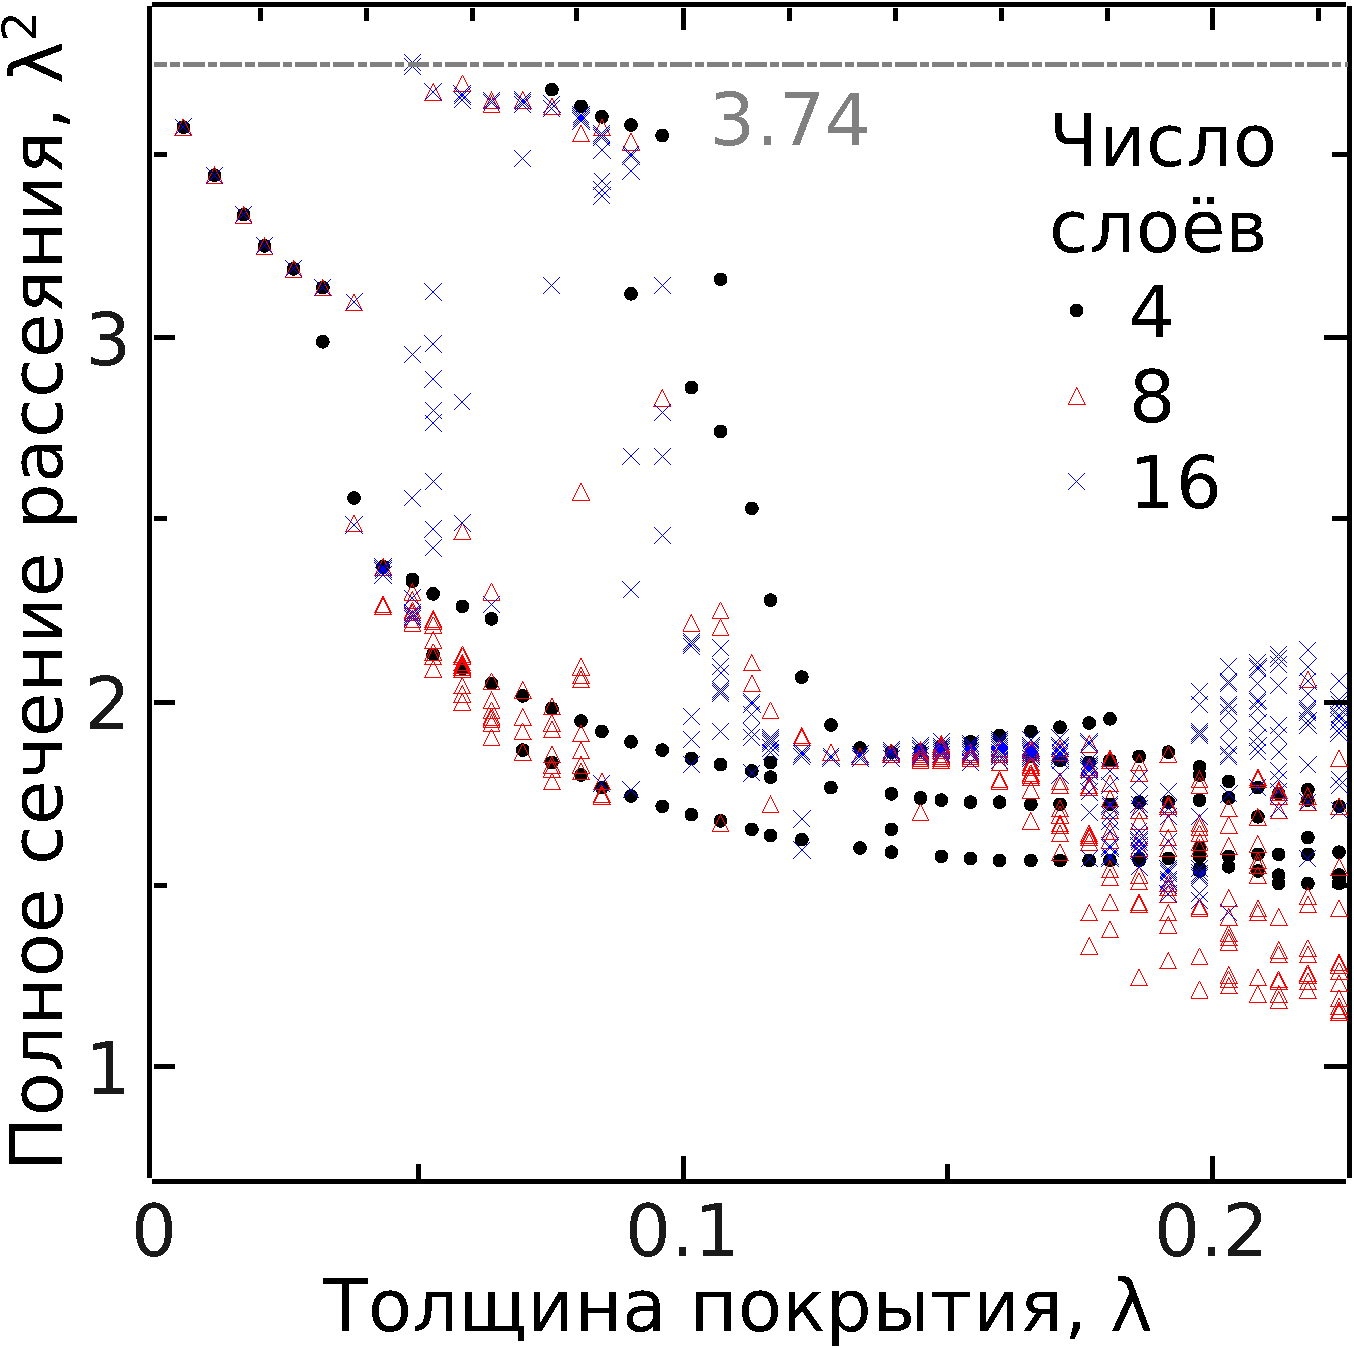
\includegraphics[width=0.95\linewidth]{rcs-overview-index07-color} \\ а)}
  \end{minipage}
  \hfill
  \begin{minipage}{0.49\linewidth}
    \centering{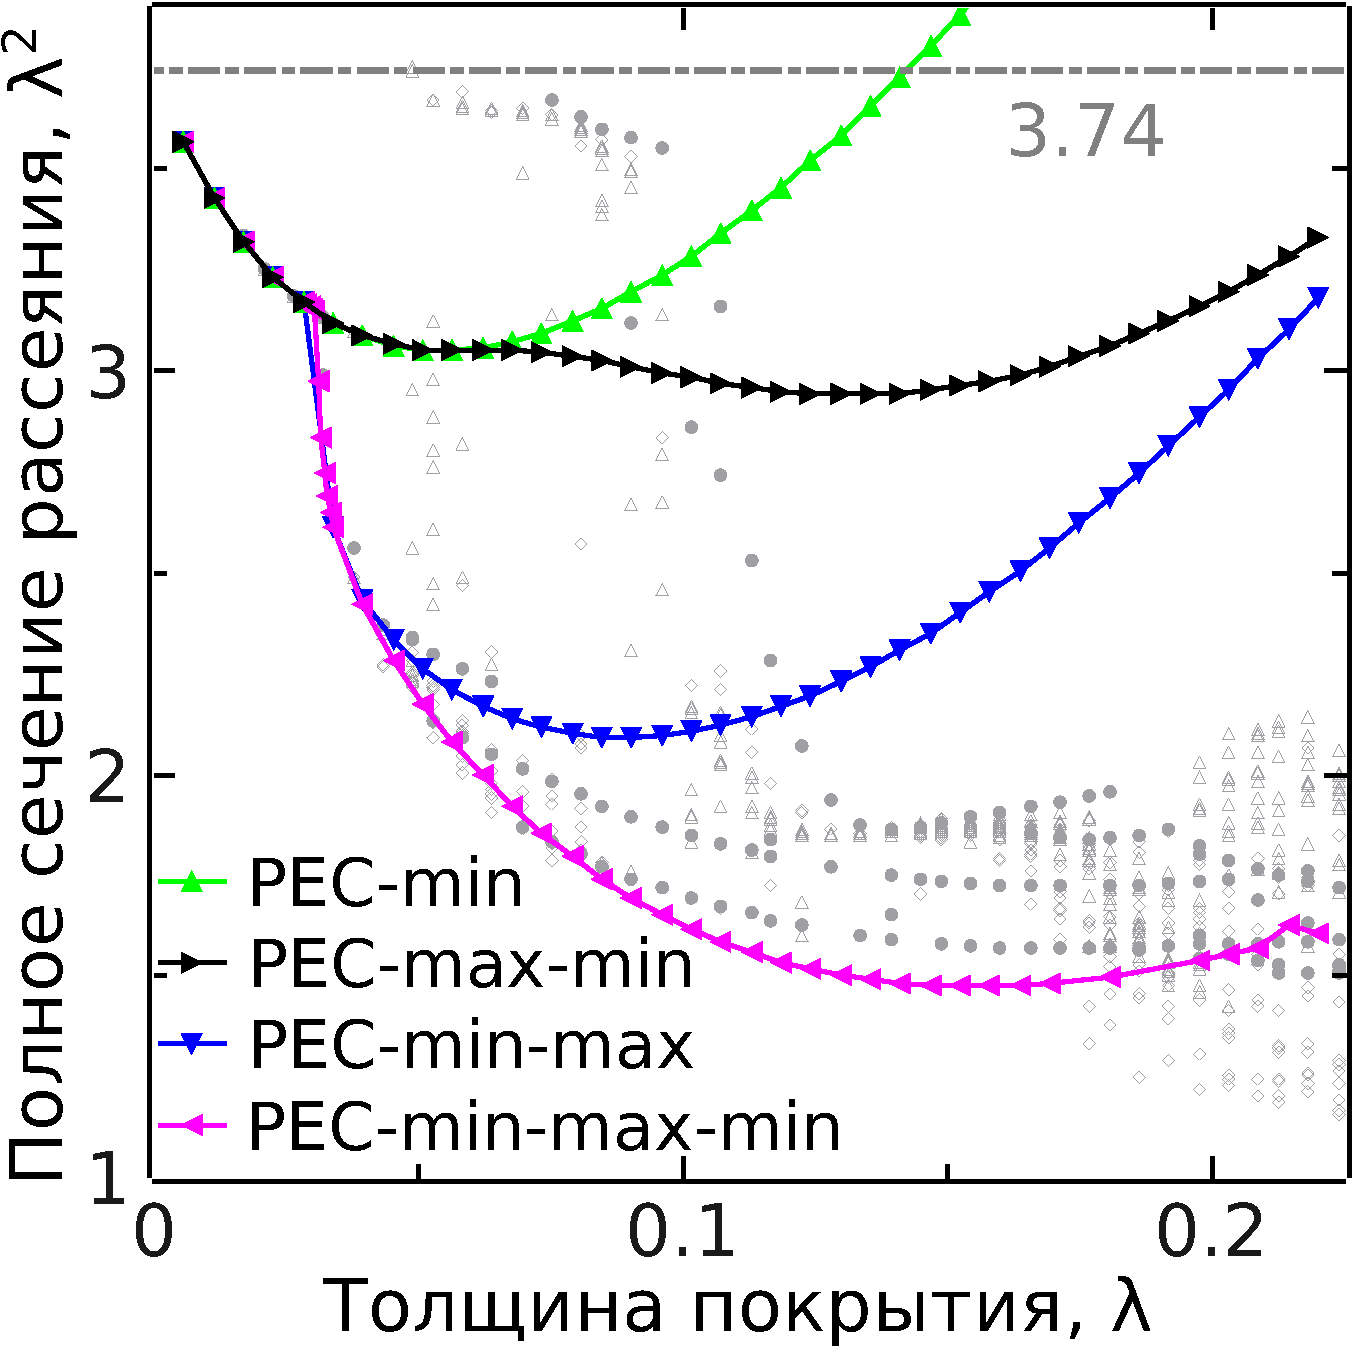
\includegraphics[width=0.95\linewidth]{rcs-overview-index07-DI} \\ б)}
  \end{minipage}
  \end{minipage}\\
  % \caption{}
  % \label{img:index07}
  \vspace*{4ex}% этим подтягиваем повыше
  % \vfill
  \\
  \begin{minipage}{\linewidth}
  \begin{minipage}{0.49\linewidth}
    \centering{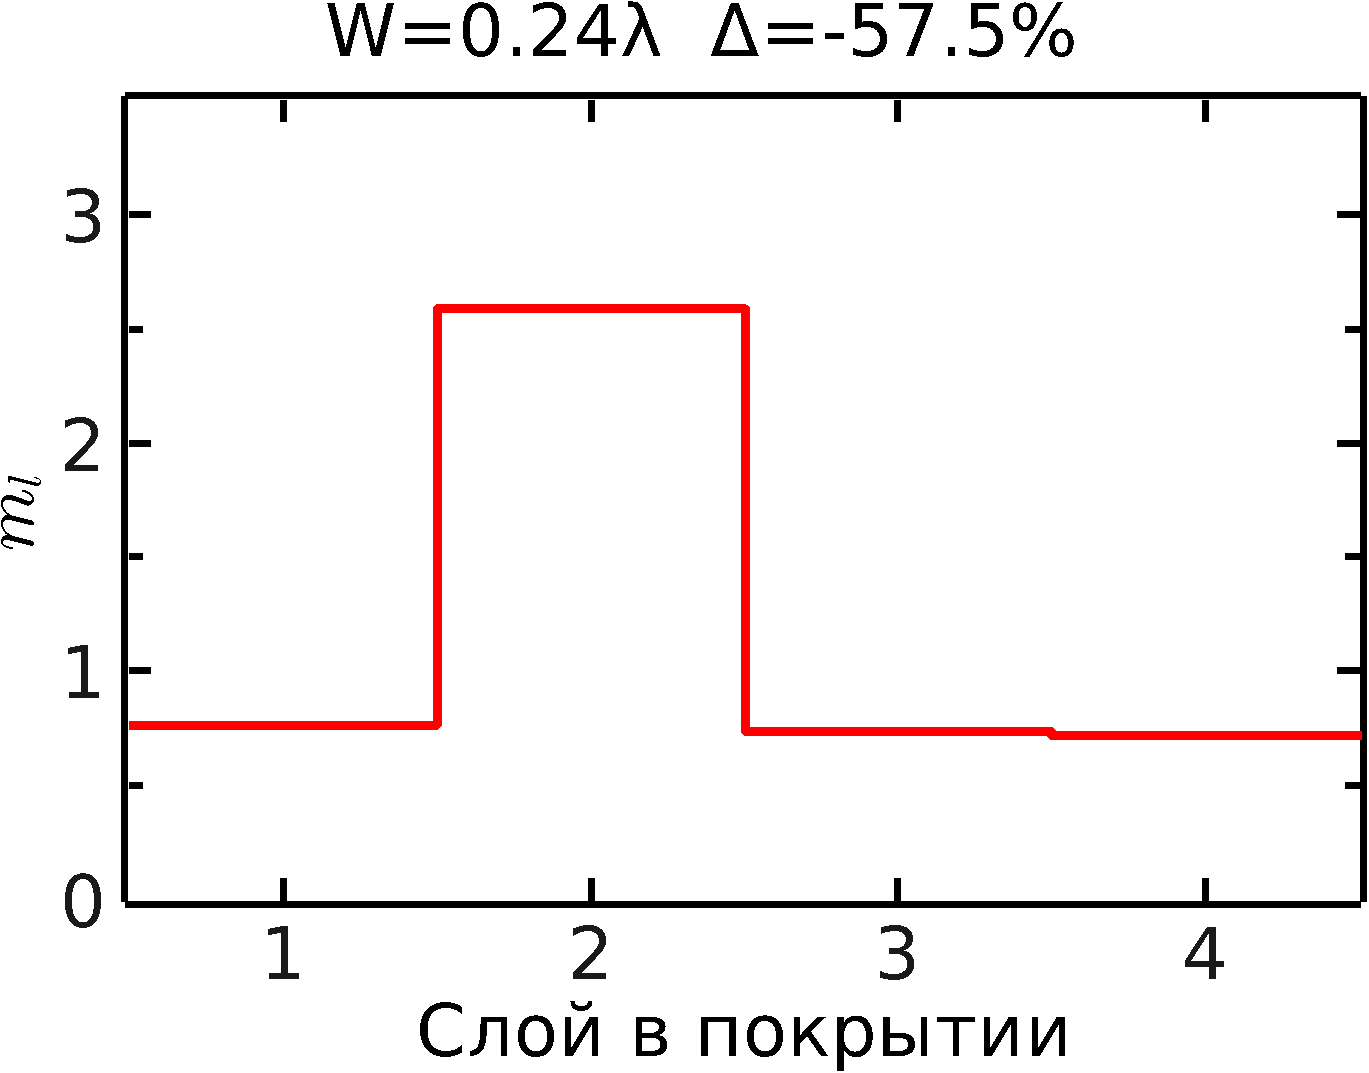
\includegraphics[width=0.91\linewidth]{index07-TO-dis} \\ в)}
  \end{minipage}
  \hfill
  \begin{minipage}{0.49\linewidth}
    \centering{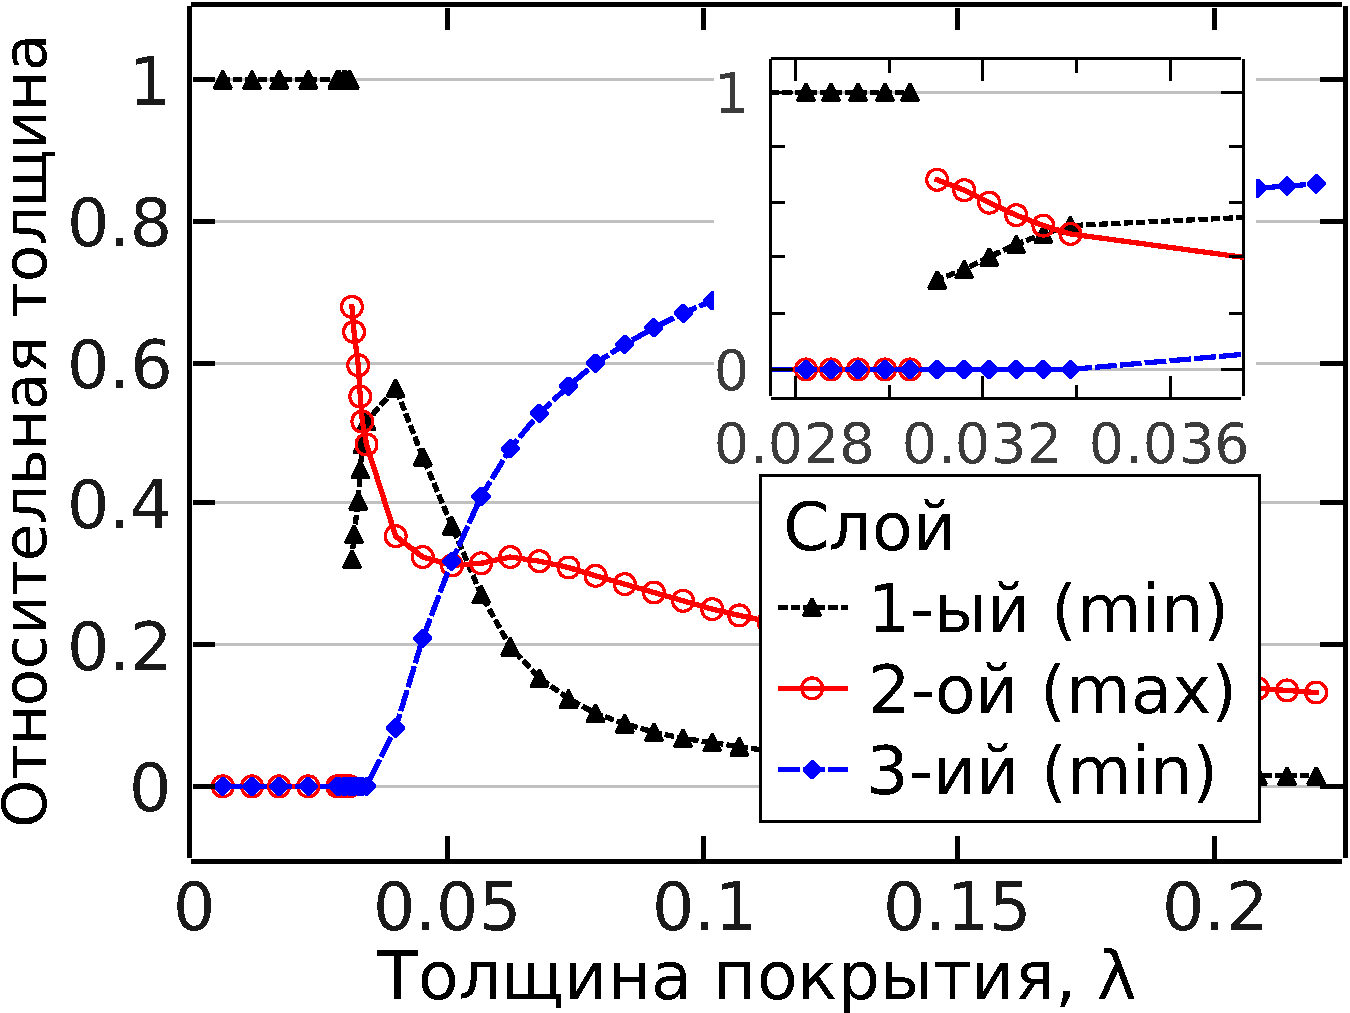
\includegraphics[width=0.95\linewidth]{index07-width} \\ г)}
  \end{minipage}
  \end{minipage}
  \caption{Результат оптимизации а) показателей преломления в каждом
    слое при его фиксированой толщине и б) толщины каждого слоя для
    покрытий с чередующимися слоями из большого $\varepsilon$ и
    ${\varepsilon<1}$. в) Характерный дизайн покрытия для
    $n_{min} = 0.67$. г) Зависимости относительной толщины каждого
    слоя от общей толщины покрытия PEC-min-max-min. }
  \label{img:min-max-min}  
\end{figure}

В качестве примера, далее для расчётов использовалось значение
$n_{min}=0.67$, что приблизительно соответствует наличию воздушного
зазора внутри кварцевых и других стёкол или, например, в объёме,
заполненном маслом или специальным полимером.  Для такой системы была
проведена серия проходов оптимизации, итоговый результат изображён на
рисунке~\ref{img:min-max-min}(а). Как и в случае $n_{min}=1$ было
обнаружено критическое значение толщины покрытия
$W_с\approx 0.1\lambda$, после которого все получаемые дизайны
маскирующих покрытий демонстрируют приблизительно двукратное
уменьшение TSCS. Существенное отличие состоит в том, что величина
маскирующего эффекта плавно нарастает при изменении толщины покрытия
от нуля до $W_c$, а дизайны использующие всего 4 слоя ничем не
уступают покрытиям с большим числом слоёв.

Один из таких дизайнов представлен на
рисунке~\ref{img:min-max-min}(в). Он явным образом не может быть
классифицирован как одно- или двухдолинный, используемые значения
показателя преломления оказались значительно меньше $n_{max}$, а в
трёх из четырёх слоёв они приблизительно равны $n_{min}$.
Обнаруженная закономерность позволила сформулировать гипотезу,
согласно которой для создания маскирующего покрытия достаточно
использовать всего два материала: с большим $\varepsilon$ и
${\varepsilon<1}$, а в качестве параметров оптимизации можно
использовать толщину каждого слоя. Эта гипотеза была проверена
численно, результаты оптимизации для $n_{min}=0.67$ и $n_{max}=8$
представлены на рисунке~\ref{img:min-max-min}(б). Оказалось, что для
большей части рассматриваемого диапазона общей толщины покрытия
достаточно всего трёх слоёв, чтобы получить приблизительно то же
уменьшение полного сечения рассеяния, что и в случае применения 4, 8 и
16 слоёв равной толщины с оптимизацией материальных параметров каждого
слоя.

Был рассмотрен и ряд других случаев, когда покрытие использует
чередование двух материалов, чьи толщины подвергались оптимизации
(рисунок ~\ref{img:min-max-min}(б)), а так же вырожденный случай
покрытия из одного слоя заданной толщины.  Для обозначения различных
дизайнов последовательно перечислялись характеристики материала:
вначале PEC --- материал маскируемой мишени, а затем min или max,
соответственно обозначающие использование в слое материала $n_{min}$
или $n_{max}$. Таким образом, PEC-min обозначает покрытие из одного
слоя $n_{min}$, двухслойные покрытия PEC-min-max и PEC-max-min
отличаются порядком следования материалов, трехслойное покрытие
PEC-min-max-min содержит слой с высоким показателем преломления
$n_{max}$ в окружении двух слоёв $n_{min}$. Дополнительно были
оптимизированы различные варианты 4-х и 5-ти слоёв в покрытии, однако
заметного улучшения по сравнению с PEC-min-max-min они не дали.

Для покрытий толщиной $W<0.03\lambda$ оптимальным является наличие
всего одного слоя материала $n_{min}$, это приводит к тому что в
многослойных дизайнах толщина слоёв с $n_{max}$ при оптимизации
уменьшается до нуля и, соответственно, маскирующие возможности всех
вариантов дизазайна оказываются идентичными. На
рисунке~\ref{img:min-max-min}(б) видно, что при толщине покрытия
$W>0.03\lambda$ покрытия PEC-min-max и PEC-min-max-min испытавают
перегиб. Это соответствует ситуации, когда становится выгодным
использовать более одного слоя в покрытии.

Более подробна эта ситуаци представлена на
рисунке~\ref{img:min-max-min}(г), где для случая PEC-min-max-min в
зависимости от общей толщины покрытия изображена относительная толщина
каждого слоя. При $W\approx0.03\lambda$ минимальное значение TSCS,
которое оптимизатор смог получить для покрытий PEC-min и PEC-min-max
сравнивается. Так как у второго вида дизайна скорость уменьшения TSCS
при росте толщины выше, то на рисунке~\ref{img:min-max-min}(г) этой
толщине соответсвует разрыв: для $W<0.03\lambda$ меньшее TSCS
обеспечиват дизайн PEC-min, а для $W>0.03\lambda$ выигрывает дизайн
PEC-min-max. При этом, в диапазоне толщин
$0.03\lambda < W < 0.035\lambda$ дизайн PEC-min-max оказывается
выгоднее, чем дизайн PEC-min-max-min, поэтому для трёхслойного дизайна
оптимизатор уменьшает толщину наружного слоя до нуля. Для толщины
$W>0.035\lambda$ наилучшие показатели обеспечивает дизайн
PEC-min-max-min. Интересно отметить, что для значений 
$W>0.2\lambda$ толщина внутреннего слоя min состявлет менее 2\% от
общей толщины, тем не менее он позволяет получить почти в два раза
меньшее TSCS по сравнению со случаем PEC-max-min ($\sim
1.5\lambda^2$ против более $3 \lambda^2$)

\begin{figure}[t]
  \centering
    \centering{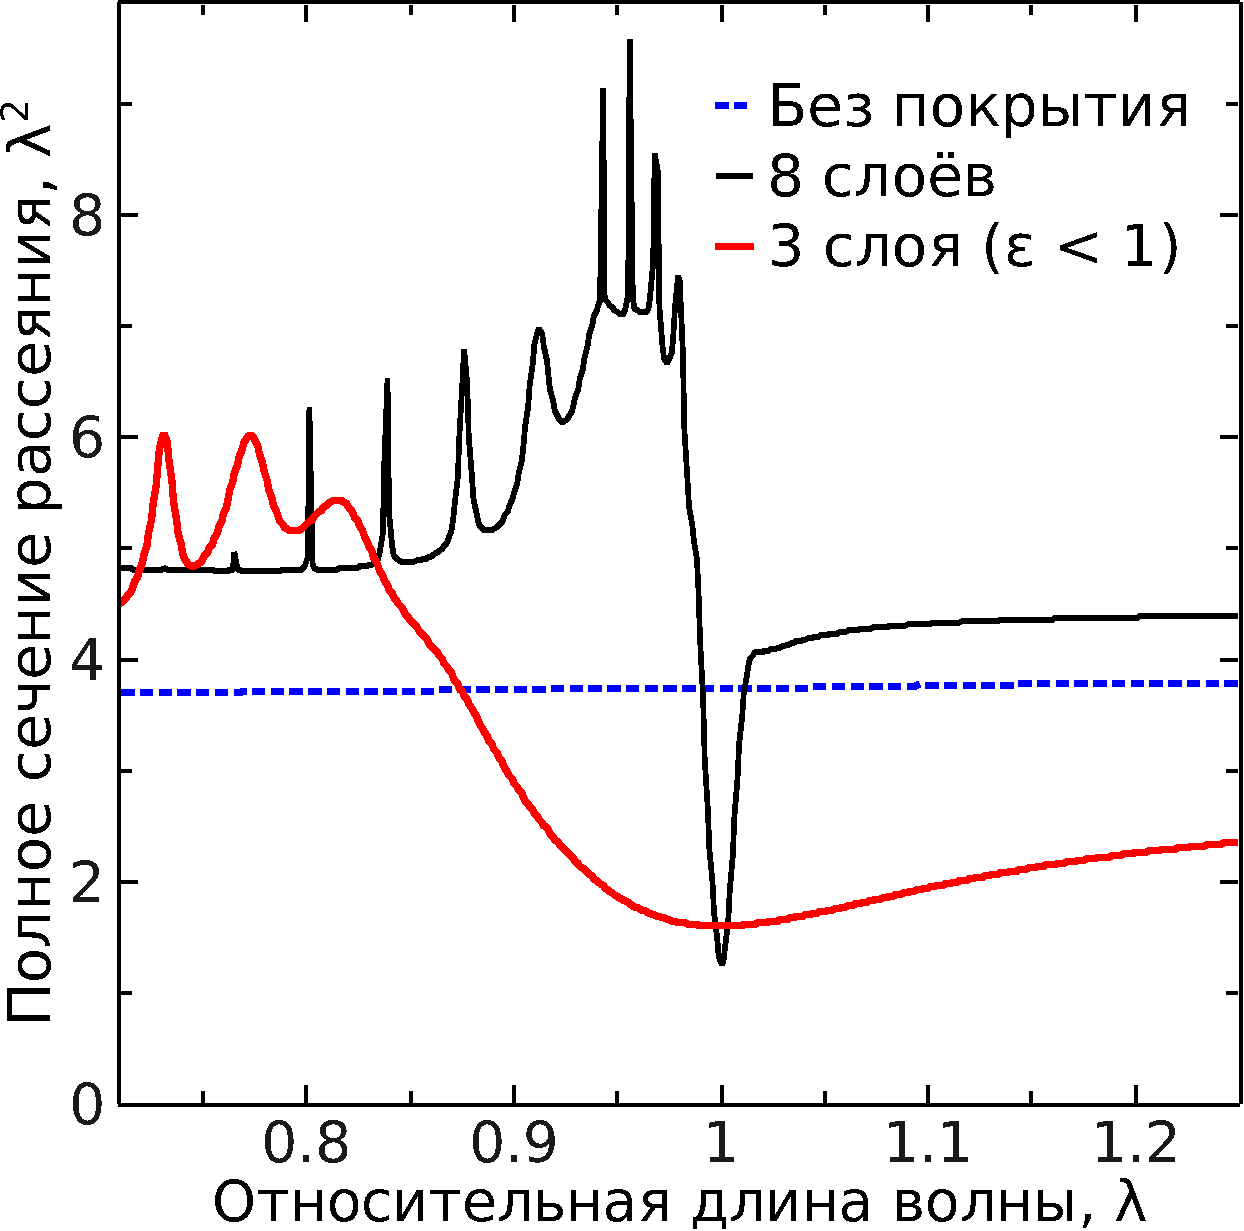
\includegraphics[width=0.55\linewidth]{index07-spectra}}
  \caption{ Спектры частицы без покрытия и с маскирующими
    покрытиями: из 8-ми слоёв диэлектрика и из 3-х слоёв с применением
    ${\varepsilon<1}$.\label{img:index07-spectra}
    }
\end{figure}
Результаты, полученые при оптимизации маскирующих сферических покрытий
можно дополнить спектрами рассеяния для случаев наличия и отсутствия
материала с ${\varepsilon<1}$ в оптимизированном покрытии.  При
расчёте спектров для рисунка~\ref{img:index07-spectra} не учитывалось
возможное наличие дисперсии и сопутствующих им потерь (обычно, они
достаточно малы для случая диэлектрических материалов), поэтому
полученая форма полностью определяется дизайном маскирующего
покрытия. Для удобства приводится спектр полученый для непокрытой PEC
мишени.  Хорошо виден относительно узкий резонанс, который определяет
маскирующие свойства покрытия из 8-ми слоёв равной
толщины. Использование материала с ${\varepsilon<1}$ позволило в
несколько раз расширить диапазон длин волн, где наблюдается подавление
рассеяния.  Такая существенная разница предполагает различные
физические механизмы, объясняющие подавление рассеяния в этих двух
случаях, что и будет рассмотрено в следующем разделе.

\section{Картина ближнего поля}\label{sec:near-field}

В предыдущих разделах численным образом исследовалось поведение
многослойных сферических покрытий из диэлектриков. Сравнение
рисунков~\ref{img:scattering}(б), \ref{img:rcs-overview-r14-42}(а--б),
изображающих достижимое уменьшение TSCS в зависимости от толщины
покрытия для трёх разных радиусов маскируемой мишени, позволяет
выявить следующие факты:
\begin{itemize}
\item Критическая толщина покрытия слабо зависит от размера мишени.
\item Относительная эффективность маскировки растёт при уменьшении
  размера мишени.
\item Эффективность маскировки оптимизрованным покрытием слабо зависит
  от выбора общей толщины покрытия после достижения критической
  величины для всех рассмотренных размеров мишени.
\end{itemize}
Моделирование дизайнов с ${\varepsilon<1}$ используя оптимизацию
толщины каждого слоя покрытия позволило сделать ещё несколько
наблюдений:
\begin{itemize}
\item Достаточно всего трёх слоёв в покрытии для достижения уровня
  маскировки сопоставимого со случаями 4, 8 и 16 слоёв равной толщины,
  где для оптимизации использвалось значение показателя преломления.
\item Использование ${\varepsilon<1}$ позволяет значительно расширить
  полосу частот, для которой наблюдается эффект маскировки,
  обусловленный наличием покрытия (рисунок~\ref{img:index07-spectra}).
\end{itemize}
Чтобы получить ответ о причинах такого поведения, необходимо
рассмотреть картины ближнего поля, представленные на
рисунках~\ref{img:field-phase} и \ref{img:field-amplitude}.

\begin{figure}[p]
  \begin{minipage}[ht]{0.495\linewidth}
    \centering{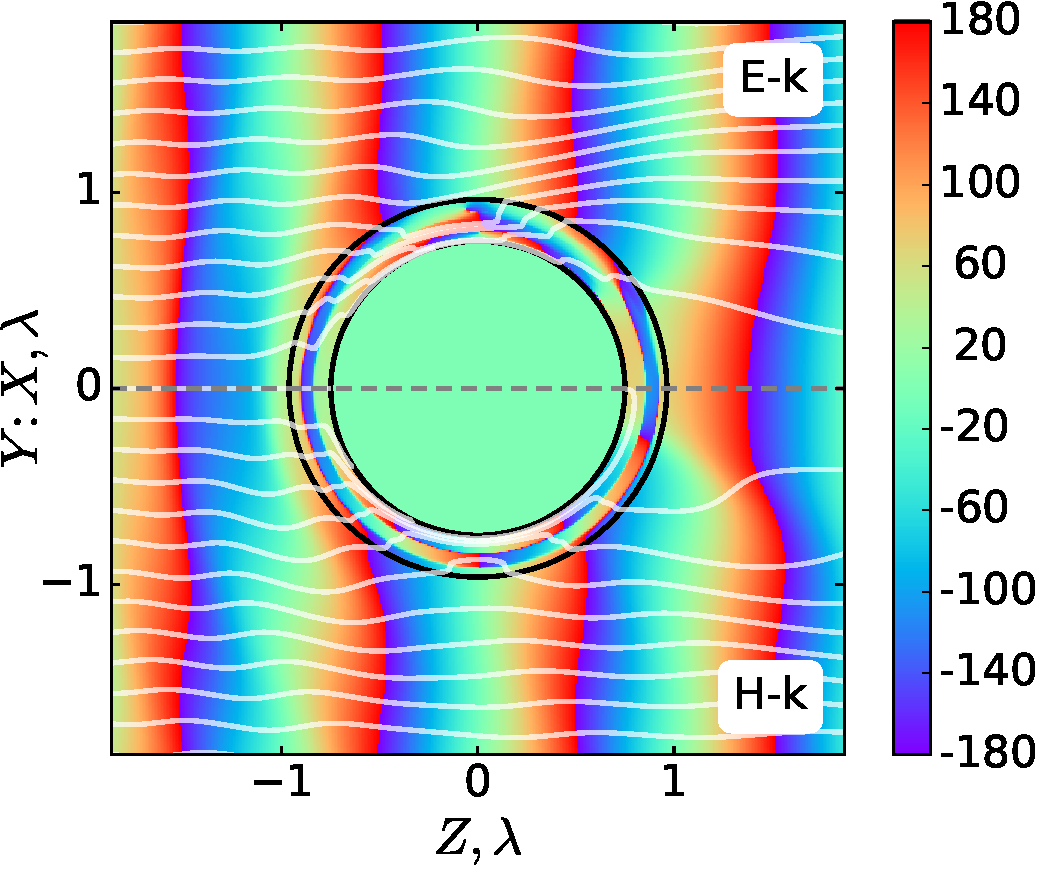
\includegraphics[width=0.98\linewidth]{PEC-index-dv-R4-XYZ-angleEx-rainbow} \\ а)}
  \end{minipage}
  \hfill
  \begin{minipage}[ht]{0.495\linewidth}
    \centering{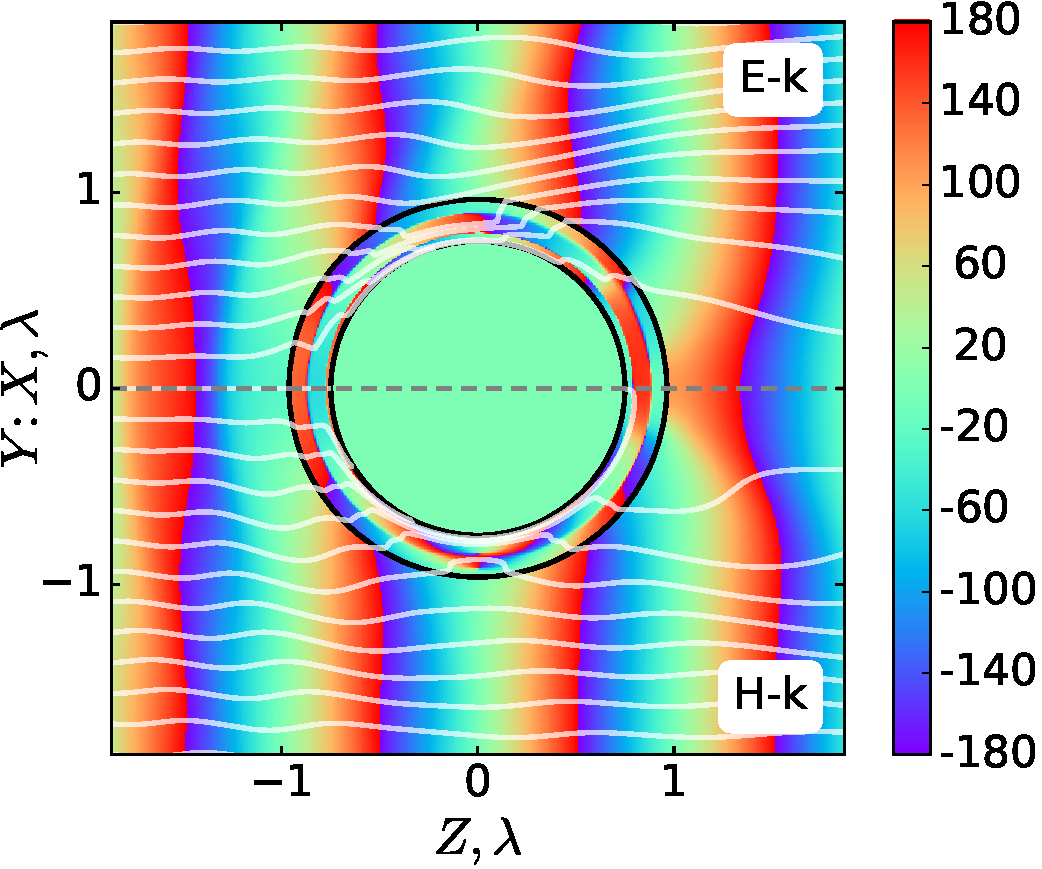
\includegraphics[width=0.98\linewidth]{PEC-index-dv-R4-XYZ-angleHy-rainbow} \\ б)}
  \end{minipage}
  \begin{minipage}[ht]{0.495\linewidth}
    \centering{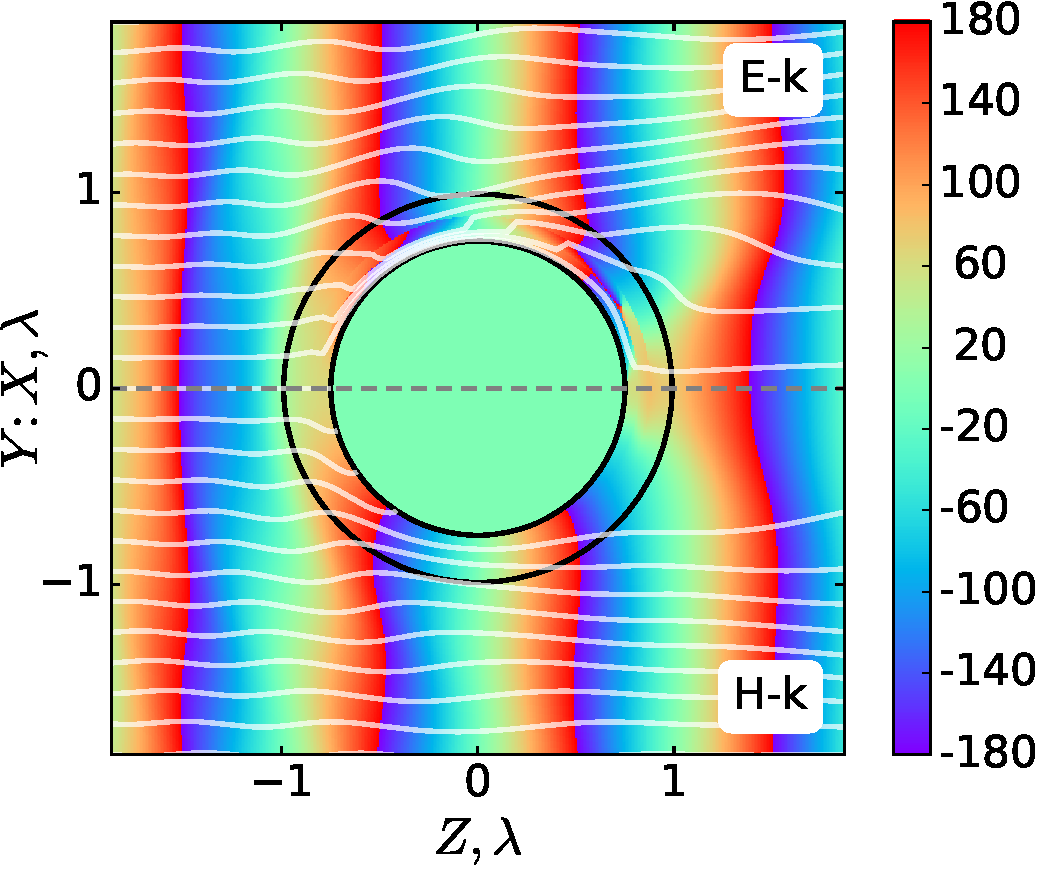
\includegraphics[width=0.98\linewidth]{PEC-index-in-glass-R4-XYZ-angleEx-rainbow} \\ в)}
  \end{minipage}
  \hfill
  \begin{minipage}[ht]{0.495\linewidth}
    \centering{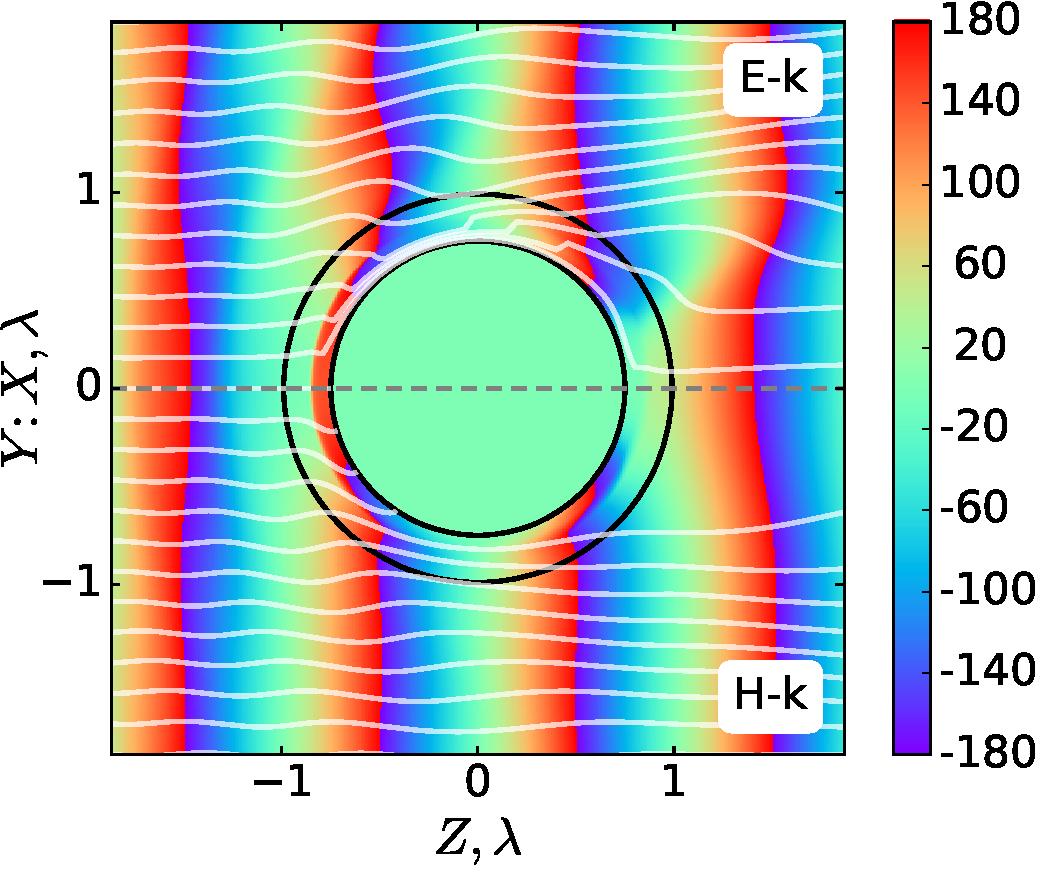
\includegraphics[width=0.98\linewidth]{PEC-index-in-glass-R4-XYZ-angleHy-rainbow} \\ г)}
  \end{minipage}

  \caption{Изображение фазы электрического (а,в) и магнитного (б,г)
    поля в случае маскировки объекта покрытием из изотропных
    диэлектриков ( а,б, см.~рисунок~\ref{img:designs}(а)) и материалов
    с ${\varepsilon <1}$ (в,г,
    см.~рисунок~\ref{img:min-max-min}(в)). Изображения построены в
    виде эпюра из плоскости поляризации падающей волны (E-k, верхняя
    половина) и перпендикулярной плоскости (H-k, нижняя половина). Чёрные
    окружности маркируют границы маскирующего покрытия. Белым
    обозначены линии потока энергии, волна распространяется в
    плоскости рисунка слева направо.}
  \label{img:field-phase}
\end{figure}

\begin{figure}[p]
  \begin{minipage}[ht]{0.495\linewidth}
    \centering{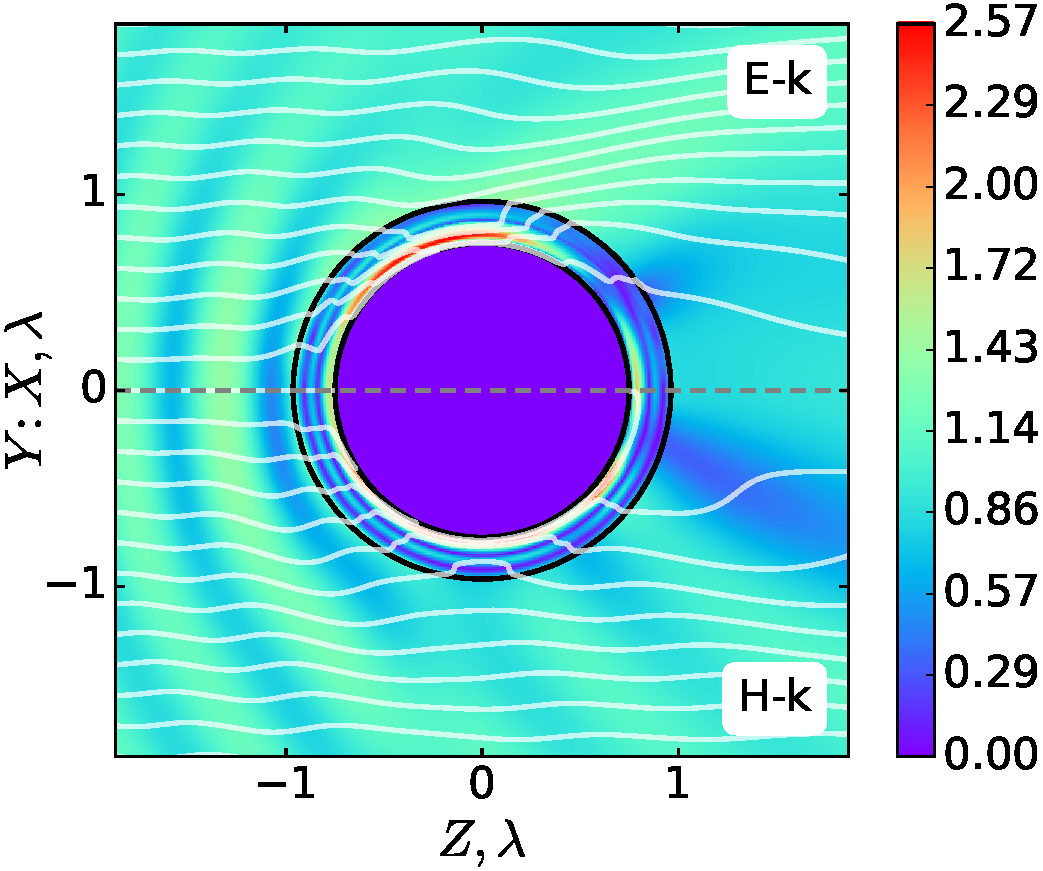
\includegraphics[width=0.98\linewidth]{PEC-index-dv-R4-XYZ-Eabs} \\ а)}
  \end{minipage}
  \hfill
  \begin{minipage}[ht]{0.495\linewidth}
    \centering{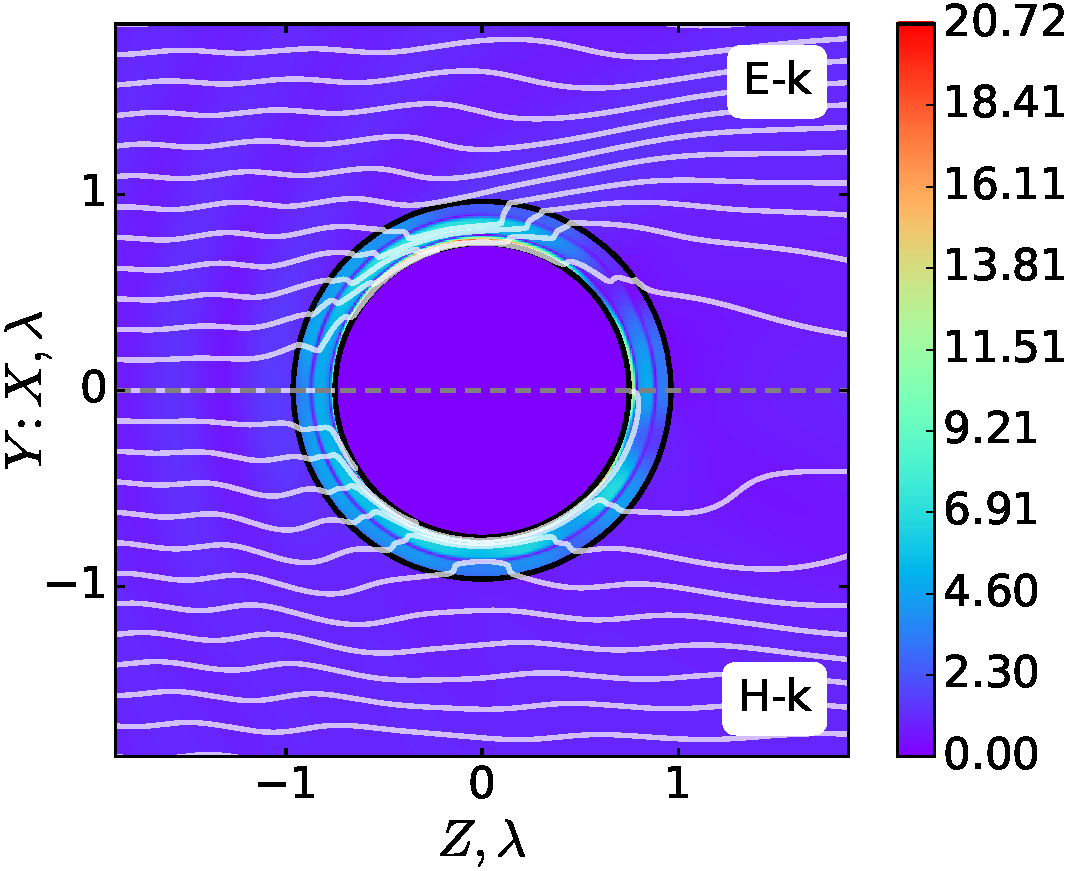
\includegraphics[width=0.98\linewidth]{PEC-index-dv-R4-XYZ-Habs-full} \\ б)}
  \end{minipage}
  \begin{minipage}[ht]{0.495\linewidth}
    \centering{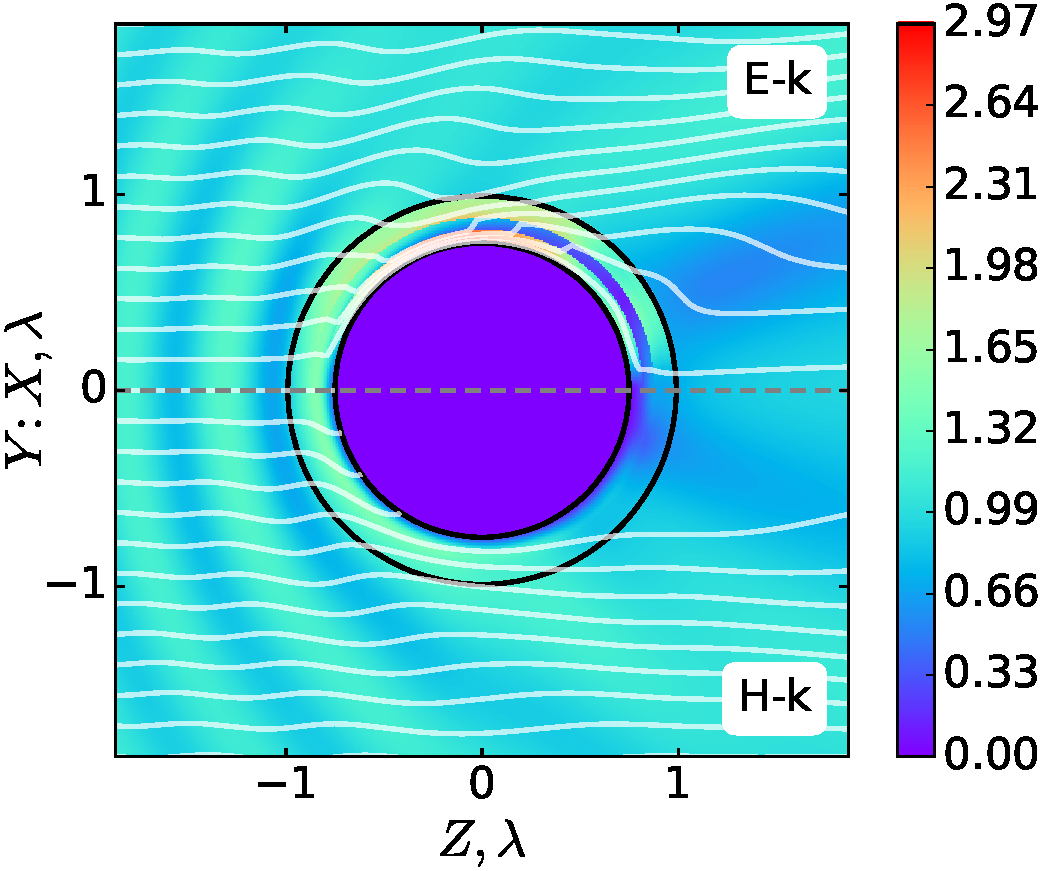
\includegraphics[width=0.98\linewidth]{PEC-index-in-glass-R4-XYZ-Eabs-full} \\ в)}
  \end{minipage}
  \hfill
  \begin{minipage}[ht]{0.495\linewidth}
    \centering{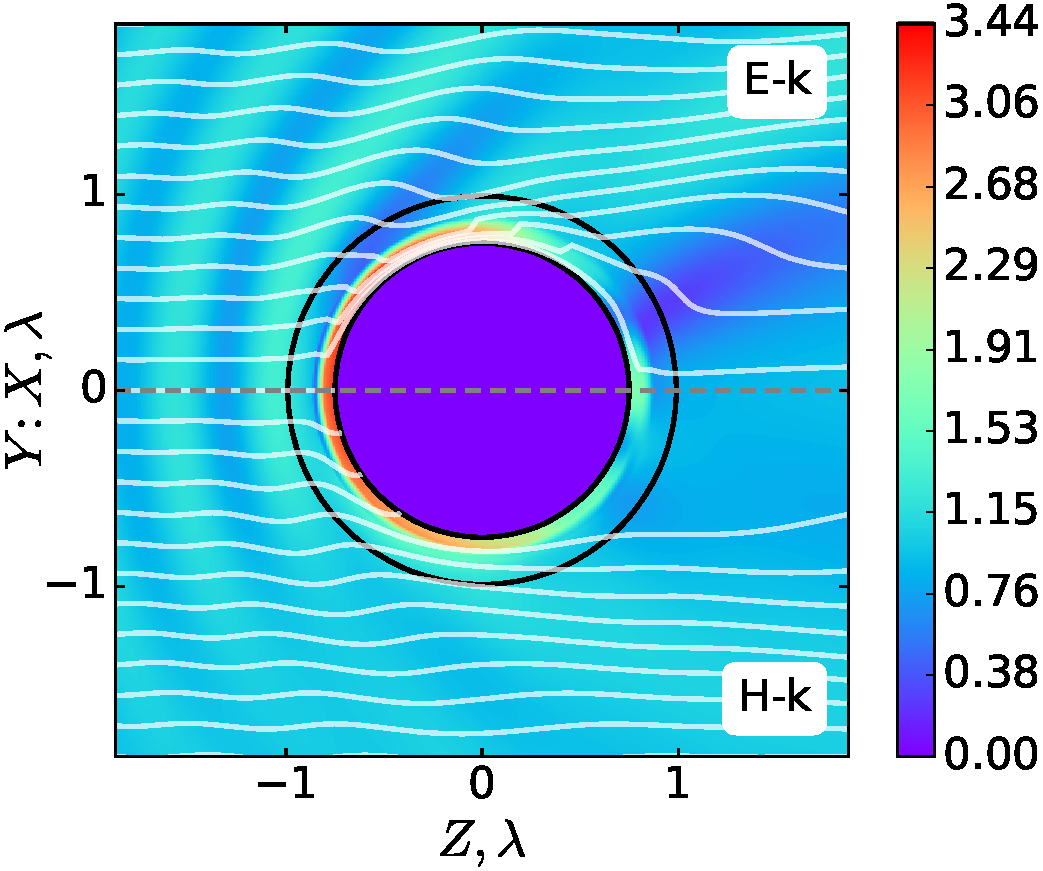
\includegraphics[width=0.98\linewidth]{PEC-index-in-glass-R4-XYZ-Habs-full} \\ г)}
  \end{minipage}

  \caption{Аналогично рисунку~\ref{img:field-phase} для амплитуды
    электрического (а,в) и магнитного (б,г) поля в случае маскировки
    объекта покрытием из изотропных диэлектриков ( а,б,
    см.~рисунок~\ref{img:designs}(а)) и материалов с
    ${\varepsilon <1}$ (в,г,
    см.~рисунок~\ref{img:min-max-min}(в)). Амплитуда магнитного поля
    была домножена на импеданс свободного пространства. Изображения
    построены в виде эпюра из плоскости поляризации падающей волны
    (E-k, верхняя половина) и перпендикулярной плоскости (H-k, нижняя
    половина). Чёрные окружности маркируют границы маскирующего
    покрытия. Белым обозначены линии потока энергии, волна
    распространяется в плоскости рисунка слева направо.}
  \label{img:field-amplitude}
\end{figure}

Можно отметить несколько особенностей распределения поля внутри
покрытия из изотропных диэлектриков. 1) Электромагнитное поле в
основном сконцентрировано во внутренних слоях покрытия. 2)
Присутствует нечто вроде антикорреляции между минимумами и максимумами
пространственного распределения амплитуд электрического и магнитного
полей: максимум электрического поля соответствует минимуму магнитного
и наоборот. 3) Существуют тонкие <<переключающие>> слои с быстрым
изменением фазы.  Прохождение волны сквозь эти слои в радиальном
направлении приводит к перевороту её фазы на половину периода, далее
идёт толстый слой перевёрнутой фазы.  Положение <<переключающих>>
слоёв совпадает с минимумами амплитуды того поля, чья фаза
переворачивается.

Всё вместе это позволяет описать физический механизм, приводящий к
уменьшению рассейяния при использовании маскирующих покрытий из
изотропных диэлектриков. Для этого необходимо проследить за
электрическим и магнитным полем, проходящим через <<переключающие>>
слои.  Такие слои можно эффективно рассматривать как области резкого
замедления распространения поля, причиной которого является
интерференция падающей и рассеянной волны.  Кроме того, поверхность
постоянной фазы в области между <<переключающими>> слоями имеет
предпочтительное направление движения в тангенциальном направлении.
Таким образом, один из возможных путей, по которому может пойти
падающая волна, выглядит следующим образом: волна замедляется при
прохождении сквозь <<переключающий>> слой, далее она движется в
направлении близком к тангенциальному вдоль этого слоя, замедляется
ещё раз, проходя <<переключающий>> слой в обратном направлении, и
покидает покрытие.  Вследствие использованного дизайна показателя
преломления набег фазы волны, проходящей внутри покрытия, относительно
волны, которая двигалась снаружи, оказывается в точности равен полному
периоду волны.  В результате поле, которое распространялось подобным
образом, не возмущает плоскость постоянной фазы за мишенью.

Такой механизм распространения электромагинтной волны внутри покрытия
лучше всего виден для фазы магнитного поля в плоскости поляризации и
для фазы электрического поля в перпендикулярной плоскости. Дизайн
маскирующего покрытия формирует резонатор, которой выступает в роли
волновода, направляющего распространение света вокруг мишени. Волна,
которая входит или выходит из такого резонатора, испытывает при этом
частичное отражение, тем самым не позволяя достичь идеальной
маскировки. В частности, это приводит к формированию стоячей волны,
которая даёт весомый вклад в общую картину поля внутри покрытия, а
именно из-за неё происходит существенное рассогласование фазы между
электрическим и магнитным полем. Кроме того, частичное отражение
хорошо видно на распределении для амплитуды электрического поля на
рисунке~\ref{img:field-amplitude}(а).  для интенсивности поля. Это
отражение формирует интерференционную картину при входе в покрытие, а
при выходе приводит к возникновению тени за маскируемым объектом.

Волноводоподобный характер распространения поля внутри покрытия хорошо
объясняет наличие критической толщины $W_c$, которая необходима для
возникновения маскирующего эффекта: при меньших толщинах волна
перестаёт удерживаться покрытием. Кроме того дополнительное место
необходимо для формирования согласующей части структуры, которая
позволяет полю вначале проникать внутрь, а потом покидать
покрытие. Увеличение эффективности маскировки при уменьшении размера
частицы выглядит достаточно логичным, ввиду фиксированного значения
$W_c$.  Одной и той же толщине покрытия приходится в меньшей степени
(на меньшую долю длины волны) отклонять поле, по сравнению с
невозмущённым случаем, а это, с очевидностью, сделать проще. Это
достаточно общий эффект, который наблюдается и в работах других
авторов~\cite{Alu-2005,Semouchkina-2013}.

В случае двухдолинного дизайна возникает два <<переключающих>> слоя.
Внешний слой работает аналогично тому, как было указано выше, а
внутренний слой вносит дополнительную задержку в распространиение
волны. Результирующий набег фазы волны, проходящей через внутренний
слой, оказывается равен двум периодам.  Предложенное физическое
описание механизма уменьшения полного сечения рассеяния позволяет
сделать простое предсказание.  При рассмотрении указанных дизайнов во
временной области установление стационарного распределения амплитуды
поля в области геометрической тени займёт больше времени в случае
двухдолинного дизайна по сравнению с однодолинным. Этот эффект будет
достаточно заметен, так как поле в основном концентрируется во
внутренних слоях покрытия (рисунок~\ref{img:field-amplitude}).

Маскирующий эффект, создаваемый покрытиями из изотропных диэлектриков,
можно также трактовать опираясь на теорию компенсации
рассеяния~\cite{Alu-2005, alu}.  В этой теории рассеяние на объекте
подавляется при использовании в покрытии материала с отрицательной
поляризумостью, за счёт чего удаётся занулить общий дипольный отклик
системы. В нашем случае наличие антипараллельных векторов локальной
поляризуемости вызвано наличием <<переключающих>> слоёв, приводящих к
изменению направления вектора электрического поля на противоположное.

Иначе выглядит распределение фазы электрического поля на
рисунке~\ref{img:field-phase}(б), здесь волна внутри покрытия на всей
его протяжённости движется в фазе с волной в окружающем пространстве.
Такие покрытия отличаются характерным дизайном
(рисунок~\ref{img:min-max-min}(в)), в котором один слой с высоким
показателем преломления находится между слоями с
${\varepsilon<1}$. Это позволяет волне внути покрытия распространяться
с большей скоростью, чем во вмещающей среде. Для маскировки
необходимо, чтобы поток энергии, который ранее двигался по прямой,
огибал мишень. В результате ему потребуется преодолеть большее
расстояние, но из-за возросшей скорости распространения внутри
покрытия у него появляется возможность получить фазу, близкую к фазе
волны, распространявшейся во вмещающей среде. Это, в свою очередь, и
определяет возникновение маскирующего эффекта для дизайнов с
использованием ${\varepsilon<1}$.

Основными фактором, ограничивающим маскирующие возможности этого типа
покрытия, является отражение волны при входе и выходе её из него.
Аналогично случаю покрытия, состоящего только из диэлектрических
слоёв, отражение при входе приводит к возникновению характерной
интерференционной картины (левая часть
рисунка~\ref{img:field-amplitude}(в)). Однако это отражение не
приводит к образованию стоячей волны, которая всегда сопровождается
наличием сдвига по фазе между электрической и магнитными
компонентами. В большей части покрытия фазы электрического и
магнитного поля совпадают (рисунок~\ref{img:field-phase}(в,г)), а
области существенно различной фазы локализованны вблизи левого и
правого края маскируемой частицы.

Различие в физических причинах, приводящих к образованию маскирующего
эффекта в двух типах покрытий, объясняет разницу в спектрах, которая
была представленна на рисунке~\ref{img:index07-spectra}. В оптимальном
случае для однодолинного дизайна дополнительный набег фазы внутри
покрытия из диэлектриков в точности соотвествует одному периоду
колебаний, поэтому волна из покрытия выходит в фазе с волной, которая
распространялась вне покрытия. При изменении длины волны падающего
излучения меняется скорость, с которой растёт вышеупомянутый
дополнительный набег фазы. Так как геометрические размеры покрытия не
изменяются, то это приводит к быстрой расфазировке волны на выходе с
волной из свободного пространства, что и соответствует достаточно
узкому провалу в спектре рассеяния. В случае использования материала с
${\varepsilon<1}$ без дисперсии свет внутри покрытия всегда будет
двигаться с одной и той же скоростью, попадая в фазу с невозмущённой
волной. Это приводит к значительно большей ширине спектральной
области, где наблюдается подавленное рассеяние. Значительное рассеяние
в коротковолной части спектра скорее всего связанно с повышенным
отражением при входе волны в покрытие.


сильный коэффициет усиления магнитного поля в покрытии из диэлектриков.







\section{Заключение}
Анализ этого и аналогичных графиков для других значений отношения
радиуса к длине волны~(рисунок~\ref{img:rcs-overview-r14-42}) позволил
выявить ряд характерных особенностей. Например, существует некое
пороговое значение толщины, после которого становится возможным
стабильное получение дизайнов, обеспечивающих заметное уменьшение
сечения рассеяния. При этом наилучшие показатели обеспечивают дизайны
характерной структуры, где несколько слоёв с высоким показателем
преломления окружают группу слоёв с низким показателем
преломления. Увеличение общей толщины покрытия приводит к переходу от
дизайнов с одной такой группой (рисунок~\ref{img:designs}(а)) к
дизайнам с двумя группами (рисунок~\ref{img:designs}(б)).




Адаптивный метод дифференциальной эволюции может быть успешно
использован для оптимизации полностью диэлектрических многослойных
покрытий в целях снижения рассеяния от сферических мишеней.  Были
найдены профили с оптимальным показателем преломления для различных
размеров мишени и толщин покрытия.  Были обнаружены одно- и
двухдолинные дизайны, которые оказались оптимальными для различных
геометрических параметров покрытия.  Для заданной максимальной
величины показателя преломления существует некая критическая толщина
покрытия, до который крайне тяжело найти дизайны покрытия с
маскирующим эффектом.  Для толщины покрытия больше критической
возникает переход от однодолинного дизайна к двухдолинному.  После
перехода существенного уменьшения TSCS не наблюдалось.  Мы
предполагаем, что также возможно существование многодолинных дизайнов,
однако мы не смогли их обнаружить по причине ограниченных
вычислительной мощности и времени.  Полученные дизайны дают
возможность для реализации маскировки без использования магнитных и
анизотропных метаматериалов.
   


TODO перестановки в пространстве для хаотического дизайна.

\underline{\textbf{Третья глава}} посвящена исследованию свойств
многослойных сферических маскирующих покрытий.

% ГОСТ Р 7.0.11—2011
% 5.3.9 На все иллюстрации должны быть приведены ссылки в тексте
% диссертации. При ссылке следует писать слово «Рисунок» с указанием
% его номера.

Сильной стороной теории Ми является возможность получать распределение
электрического и магнитного поля как внутри, так и вокруг изучаемой
наночастицы, вычислять значение фазы полей, а также строить линии
потока энергии.  Например, для структуры, изображённой на
рисунке~\ref{img:designs}(а), было рассчитано распределение фазы
электрического поля в окружающем частицу пространстве и внутри
покрытия (рисунок~\ref{img:field-phase}(а)).  Из рисунка видно, что
волна, проходящая через маскирующее покрытие, испытывает задержку фазы,
приблизительно равную $2\pi$. Другими словами, такой дизайн приводит к
тому, что электромагнитная волна после распространения внутри покрытия
на выходе оказывается в фазе с волной, которая двигалась в окружающем
пространстве.  Это, в свою очередь, подавляет картину интерференции в
дальнем поле и, в конечном итоге, объясняет возникающий маскирующий
эффект.

\clearpage